% !TEX root = ../gw.tex

\section{Applications and Extensions}

The basic $\GWa$ optimization can be applied to many graphics tasks and admits countless extensions to variations of the original problem.  To emphasize how \GWa fits into different pipelines, here we provide several examples of adapting \GWa to diverse matching problems, accompanied by proof-of-concept examples validating stability to these changes.

\subsection{Organizing Shape Collections}

%\suv{What does ``optimized GW objective'' mean? The argmin?}
The \GWa objective value after minimization is a \emph{distance} between metric spaces. These distances can be used for shape retrieval, search, exploration, or organization of shape databases. \GWa distances between geodesic distance matrices are isometry-invariant, popular for deformable shape retrieval~\cite{bronstein-2011,rustamov-2013}. For example, Figure~\ref{fig:shrec_mds} shows a multidimensional scaling (MDS) embedding of 80 models from four different categories in the SHREC dataset~\cite{Giorgi07} using pairwise \GWa distances. Note that models from the same class form distinct clusters.%have smaller distances among them. 

Computing pairwise \GWa distances can be prohibitively expensive for large datasets, so we leverage the observation of Rustamov et al.~\shortcite{rustamov-2013} that collections of similar 3D models can be compared to a single ``base shape.'' In this case, we use the \GWa maps $\G\!_{i,0}$ (where $0$ is the base shape) as a feature vector for shape $i$. We reproduce the result presented in the work of Rustamov et al., recovering the circular structure of meshes from a galloping horse animation sequence (Figure~\ref{fig:gallop}). Unlike Rustamov et al., however, our method does not require ground truth maps between shapes as input. 

% Such distances are used for shape retrieval; see~\cite{tangelder-2008} for a survey.  GW distances between geodesic distance matrices are isometry-invariant, popular in pipelines for deformable shape retrieval~\cite{bronstein-2011,rustamov-2013}.


%\if 0 %% COMMENTED BY GAB
\begin{figure}[t]\centering
\begin{tikzpicture}
\begin{axis}[ unit vector ratio*=1 1 1,
	view={10}{10},
height=.65\columnwidth,
yticklabel style={
        /pgf/number format/fixed,
        /pgf/number format/precision=3
},scaled y ticks=false,
xticklabel style={
        /pgf/number format/fixed,
        /pgf/number format/precision=3
},scaled x ticks=false,
zticklabel style={
        /pgf/number format/fixed,
        /pgf/number format/precision=3
},scaled z ticks=false,y dir = reverse,
line cap = round,
line join = round,
	grid=major,
	z buffer=sort,
	enlargelimits=upper,
legend style = {row sep =-.05in, inner sep = 0.01in},
legend cell align=left,
legend pos=outer north east
	]
		\addplot3[fill=blue,only marks,mark=cube*,mark size=3] 
		table [x index=0,y index=1,z index=2,col sep=comma] {figures/exploration/teddies.dat};
		\addlegendentry{\footnotesize Teddies};
		\addplot3[fill=red,only marks,mark=cube*,mark size=3] 
		table [x index=0,y index=1,z index=2,col sep=comma] {figures/exploration/humans.dat};
		\addlegendentry{\footnotesize Humans};
		\addplot3[fill=orange,only marks,mark=cube*,mark size=3] 
		table [x index=0,y index=1,z index=2,col sep=comma] {figures/exploration/fourlegged.dat};
		\addlegendentry{\footnotesize Four-legged};
		\addplot3[fill=violet,only marks,mark=cube*,mark size=3] 
		table [x index=0,y index=1,z index=2,col sep=comma] {figures/exploration/armadillo.dat};
		\addlegendentry{\footnotesize Armadillo};
\end{axis}
\end{tikzpicture}\vspace{-.1in}
\caption{MDS embedding of four classes from SHREC dataset.}
\label{fig:shrec_mds}
\end{figure}

\begin{figure}[t]\centering\pgfplotsset{scaled y ticks=false}
\begin{tikzpicture}
\begin{axis}[xlabel={\footnotesize PCA 1},ylabel={\footnotesize PCA 2},width=.75\columnwidth,height=.65\columnwidth,
xlabel near ticks,
ylabel near ticks,
line cap = round,
line join = round,
xlabel shift = 0,%-.08in,
ylabel shift = 0,%-.08in,
ymin = -.05, ymax = 1.05,xmin = -.05, xmax = 1.05,
yticklabel style={
        /pgf/number format/fixed,
        /pgf/number format/precision=3
},
scaled y ticks=false]%,legend cell align=left,legend pos = north west]
\addplot[color=blue,mark size = 1,mark=*,
nodes near coords, % Place nodes near each coordinate
    point meta=explicit symbolic, % The meta data used in the nodes is not explicitly provided and not numeric
    every node near coord/.append style={yshift=-.02in}, % Align each coordinate at the anchor 40 degrees clockwise from the right edge
   font=\tiny,text=black ] table[x index=0,y index=1,meta index = 2,col sep=comma] {figures/exploration/gallop_labels.txt};
\end{axis}
\end{tikzpicture}\vspace{-.15in}
\caption{Recovery of galloping horse sequence.\vspace{-.15in}}\label{fig:gallop}
\end{figure}
%\fi



%\vova{Note that in comparison to \cite{rustamov-2013} our exploration tool does not need input to be manifold meshes (it also works with point clouds), does not need input correspondences. A difference between shapes can be computed in Xs including correspondence computation, and one can control the tradeoff of efficiency vs quality by reducing the number of elements in the distance matrix. The method also works with intrinsic and extrinsic distances to capture various shape differences (try it). }
%
%\justin{Use Gromov-Wasserstein distances as distances.  Find $k$ nearest neighbors in a collection?}

\subsection{Supervised Matching}\label{sec:supervised_matching}

An important feature of a matching tool is the ability to incorporate user input, e.g.\ ground truth matches of points or regions.  In the \GWa framework, one way to enforce these constraints is to provide a \emph{stencil} $\bS$ specifying a sparsity pattern for the map $\G$.  Incorporating constraints in this form is as simple as replacing $\K\gets \K\otimes\bS$ in Algorithm~\ref{alg:gw} before Sinkhorn projection.

\begin{figure*}
\centering
\begin{tabular}{cc@{}cc@{}cc@{}c}
&
{\small \emph{Top}} & {\small\emph{Bottom}}&
{\small \emph{Top}} & {\small\emph{Bottom}}&
{\small \emph{Top}} & {\small\emph{Bottom}}\\
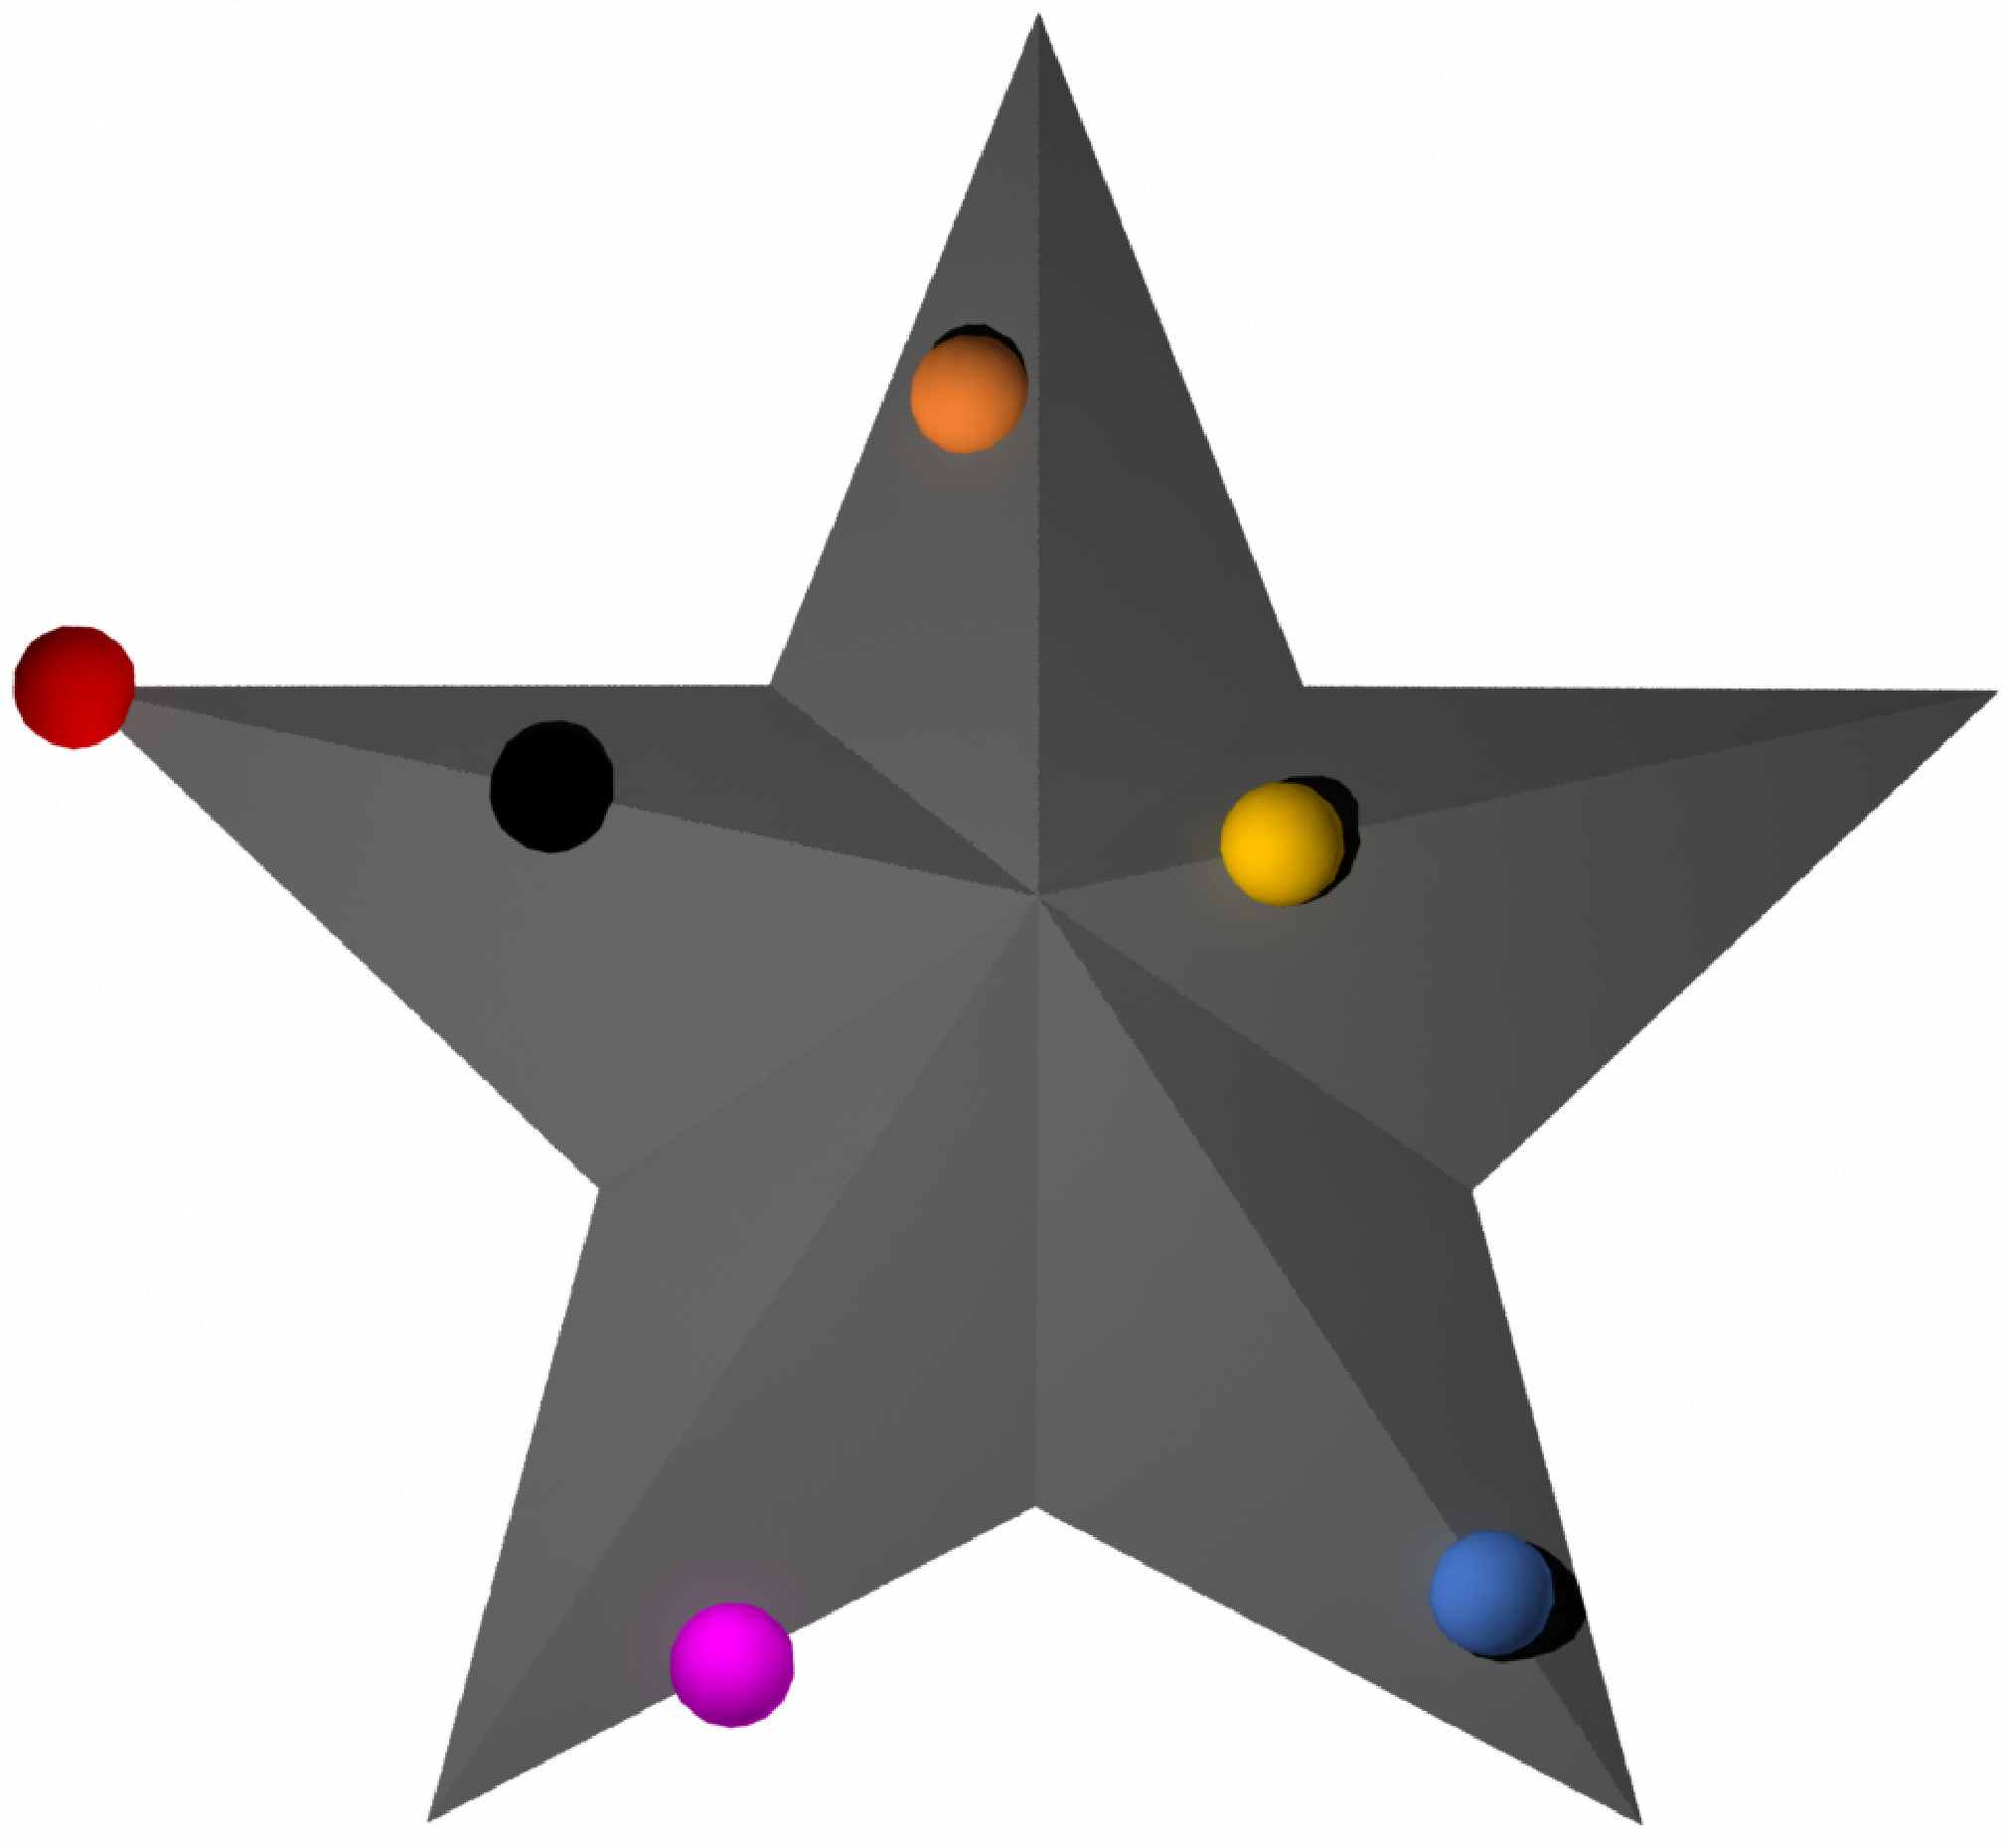
\includegraphics[height=.12\linewidth]{figures/interactive/source_surface.pdf}&
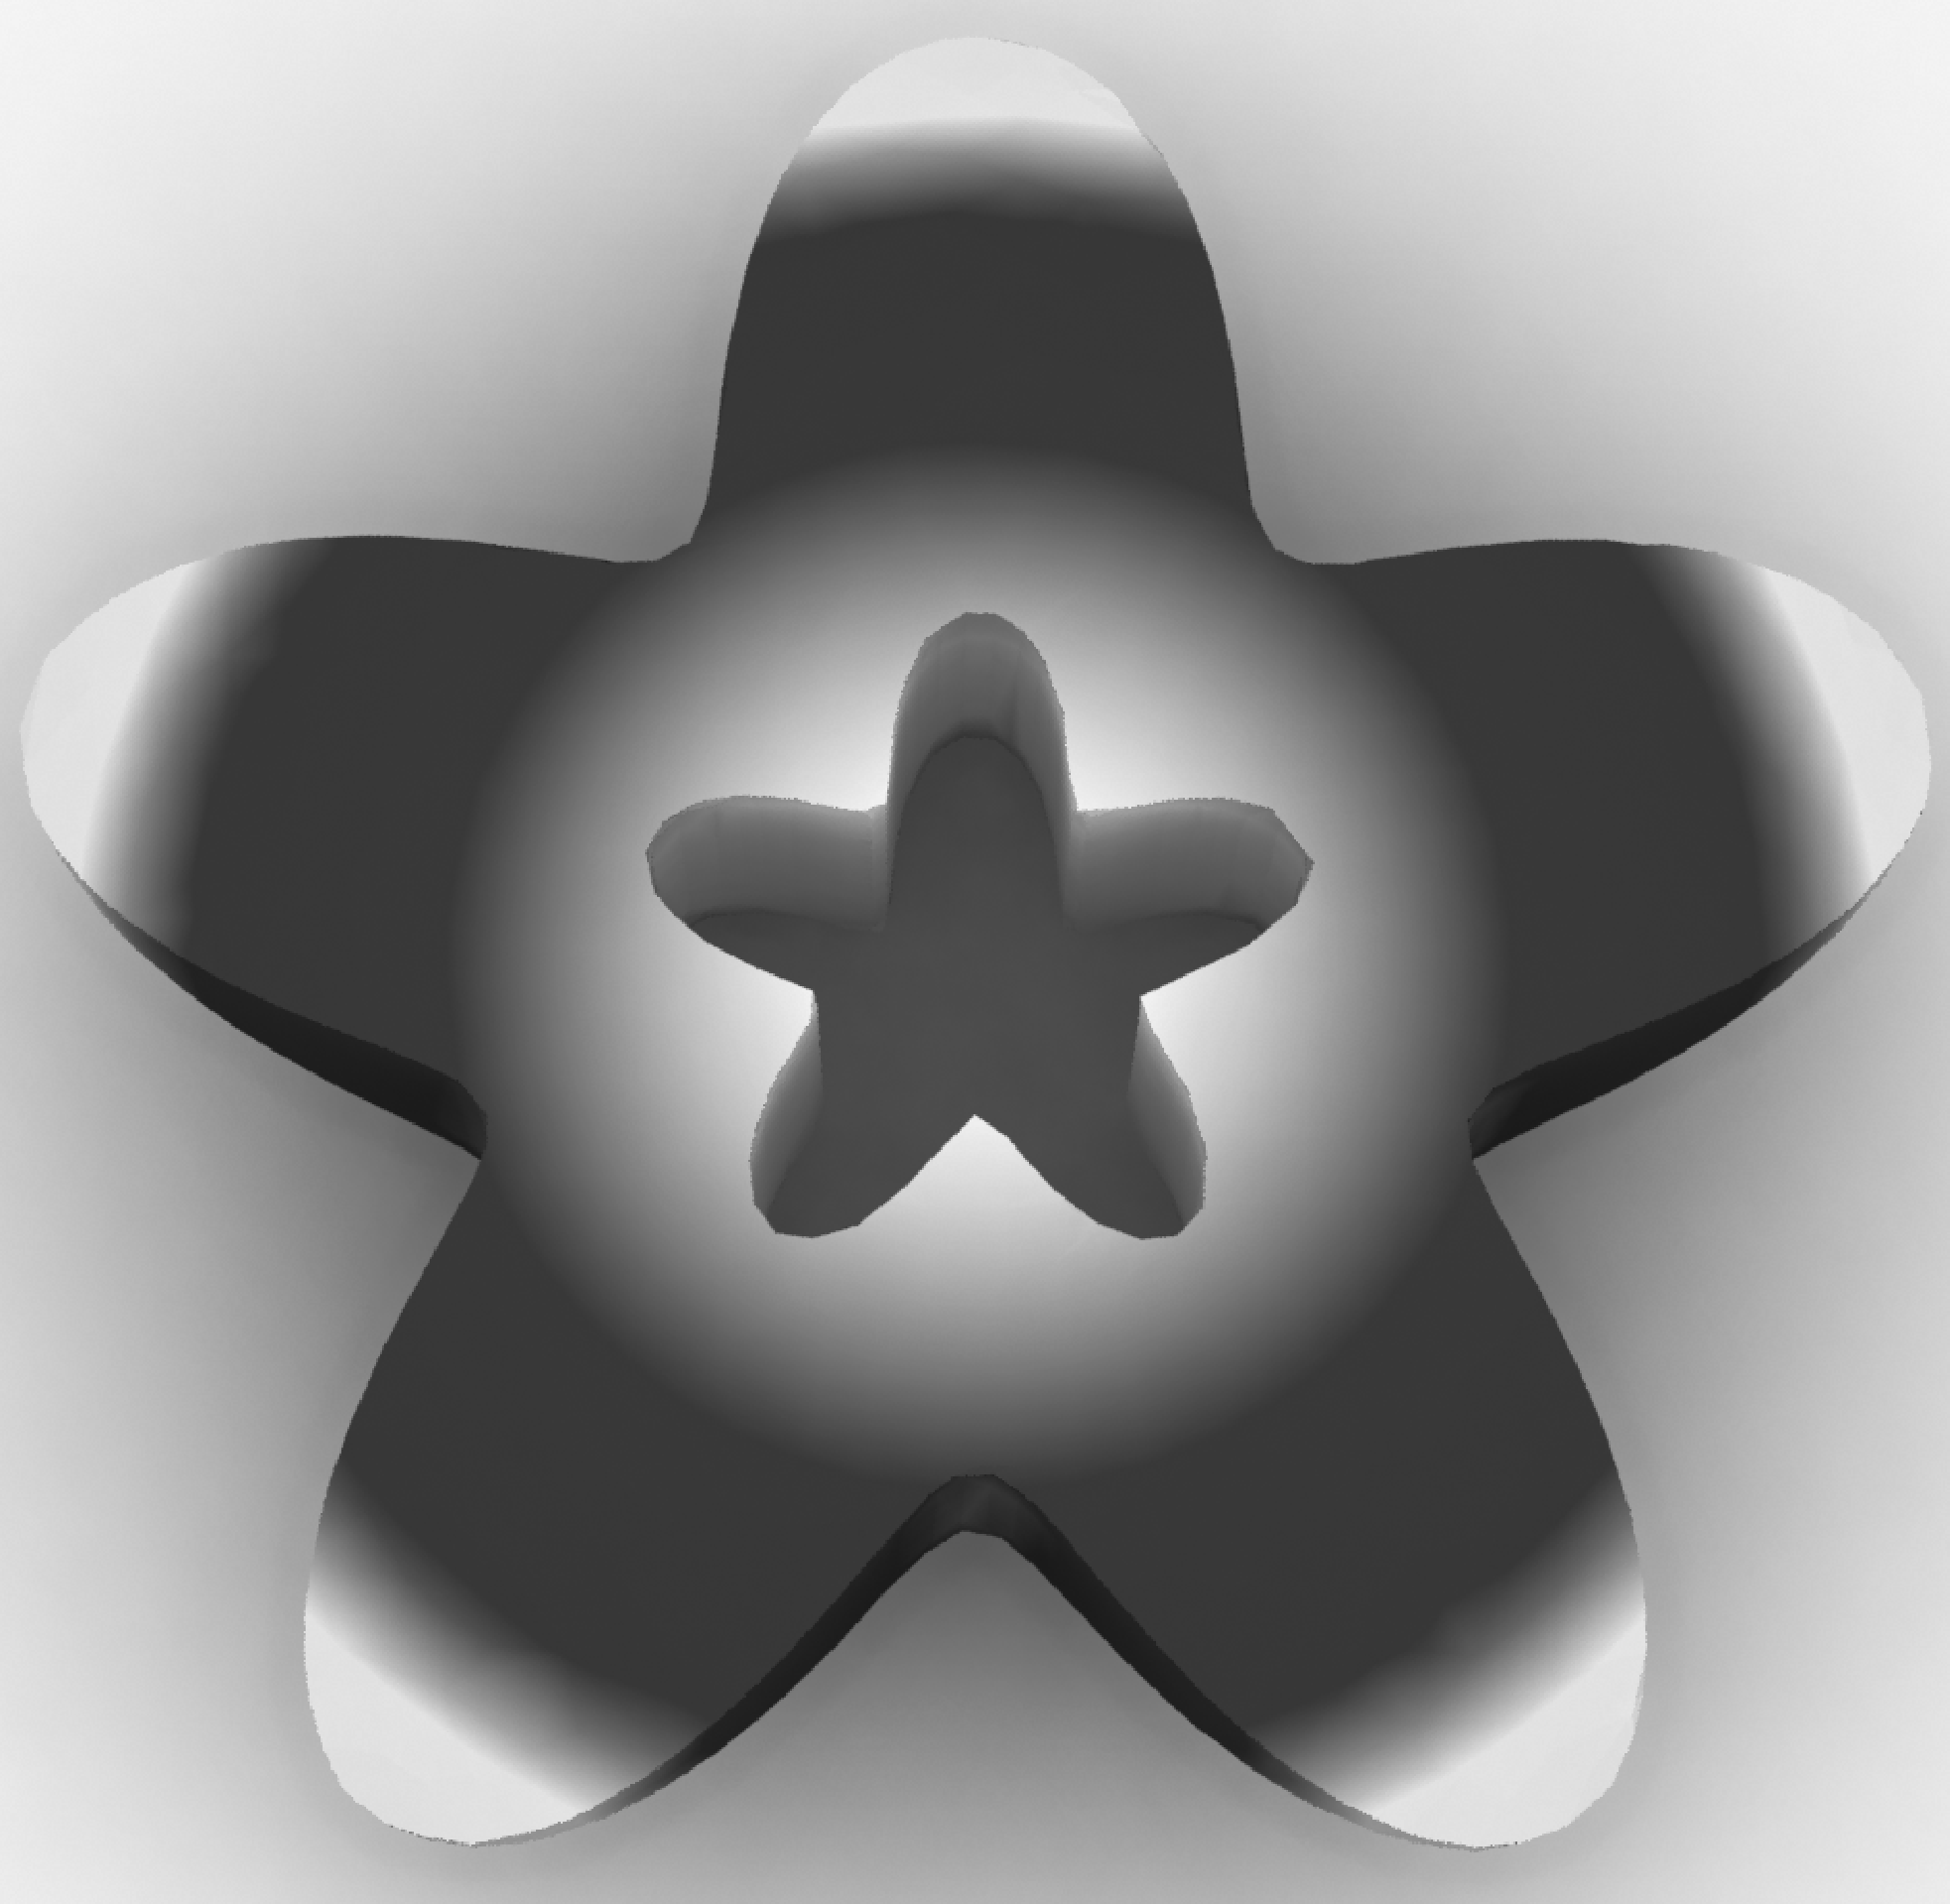
\includegraphics[height=.12\linewidth]{figures/interactive/initial_map_target_cropped.pdf}&
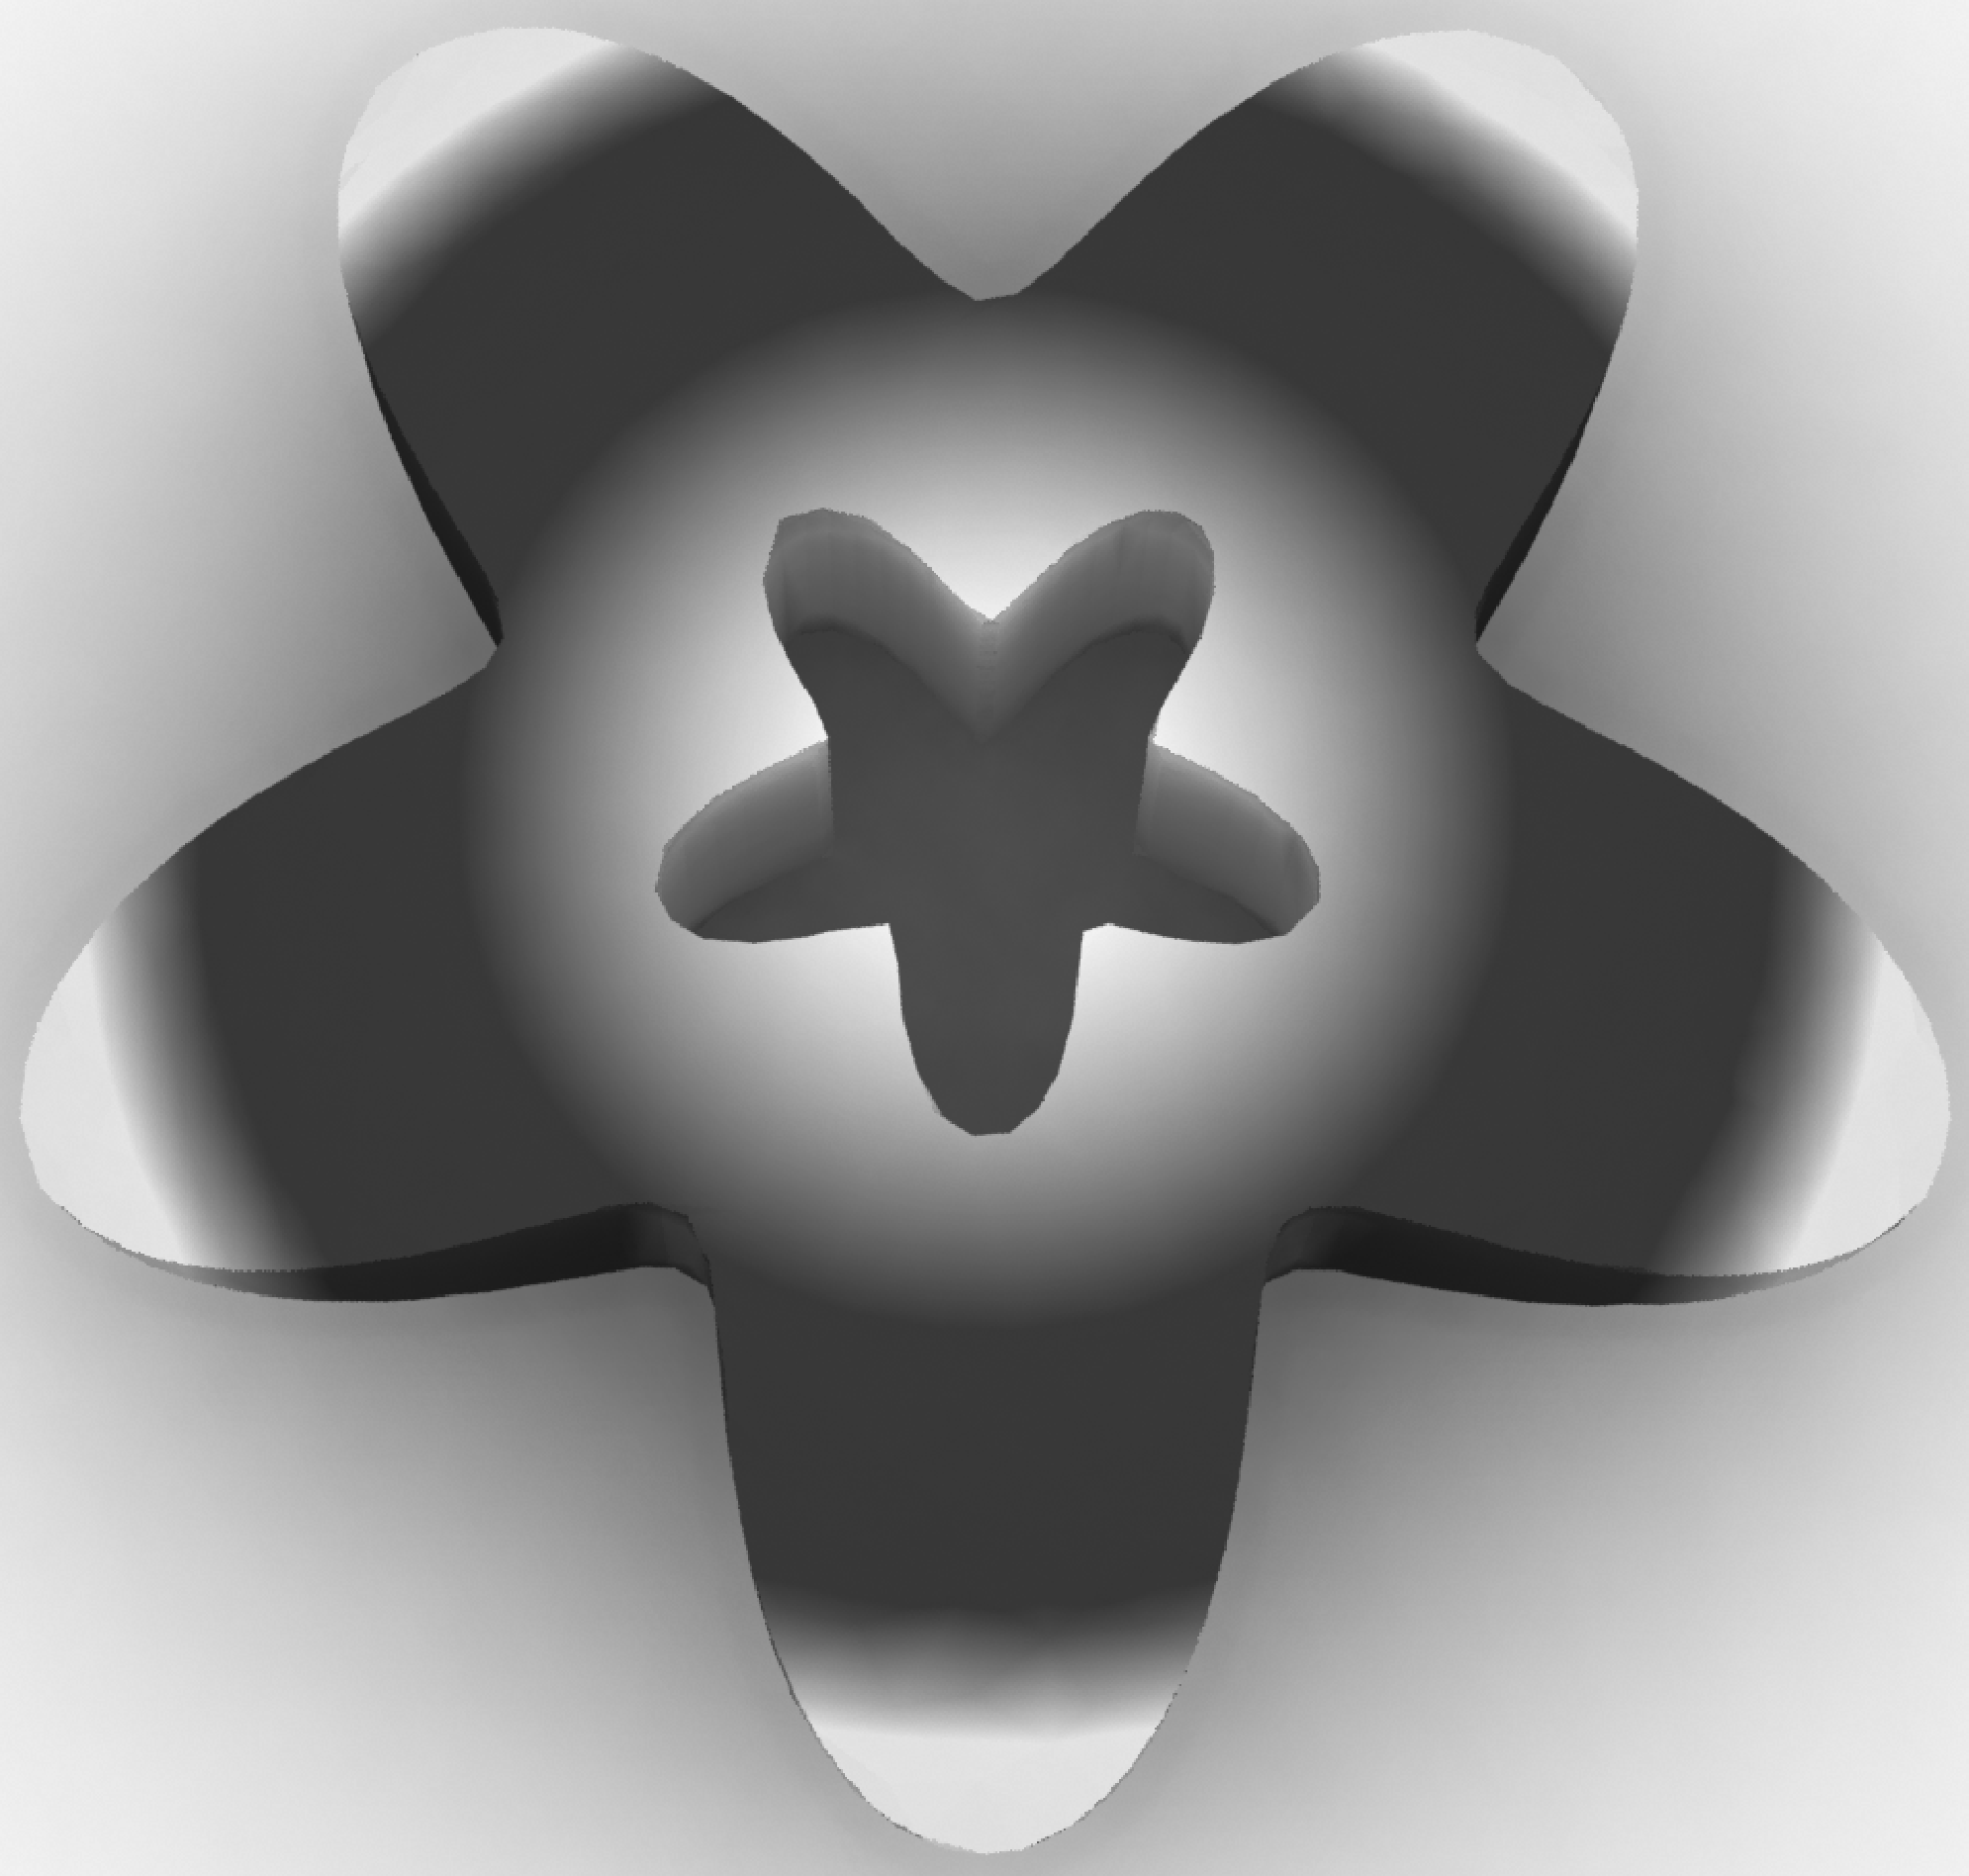
\includegraphics[height=.12\linewidth]{figures/interactive/initial_map_target_flip_cropped.pdf}&
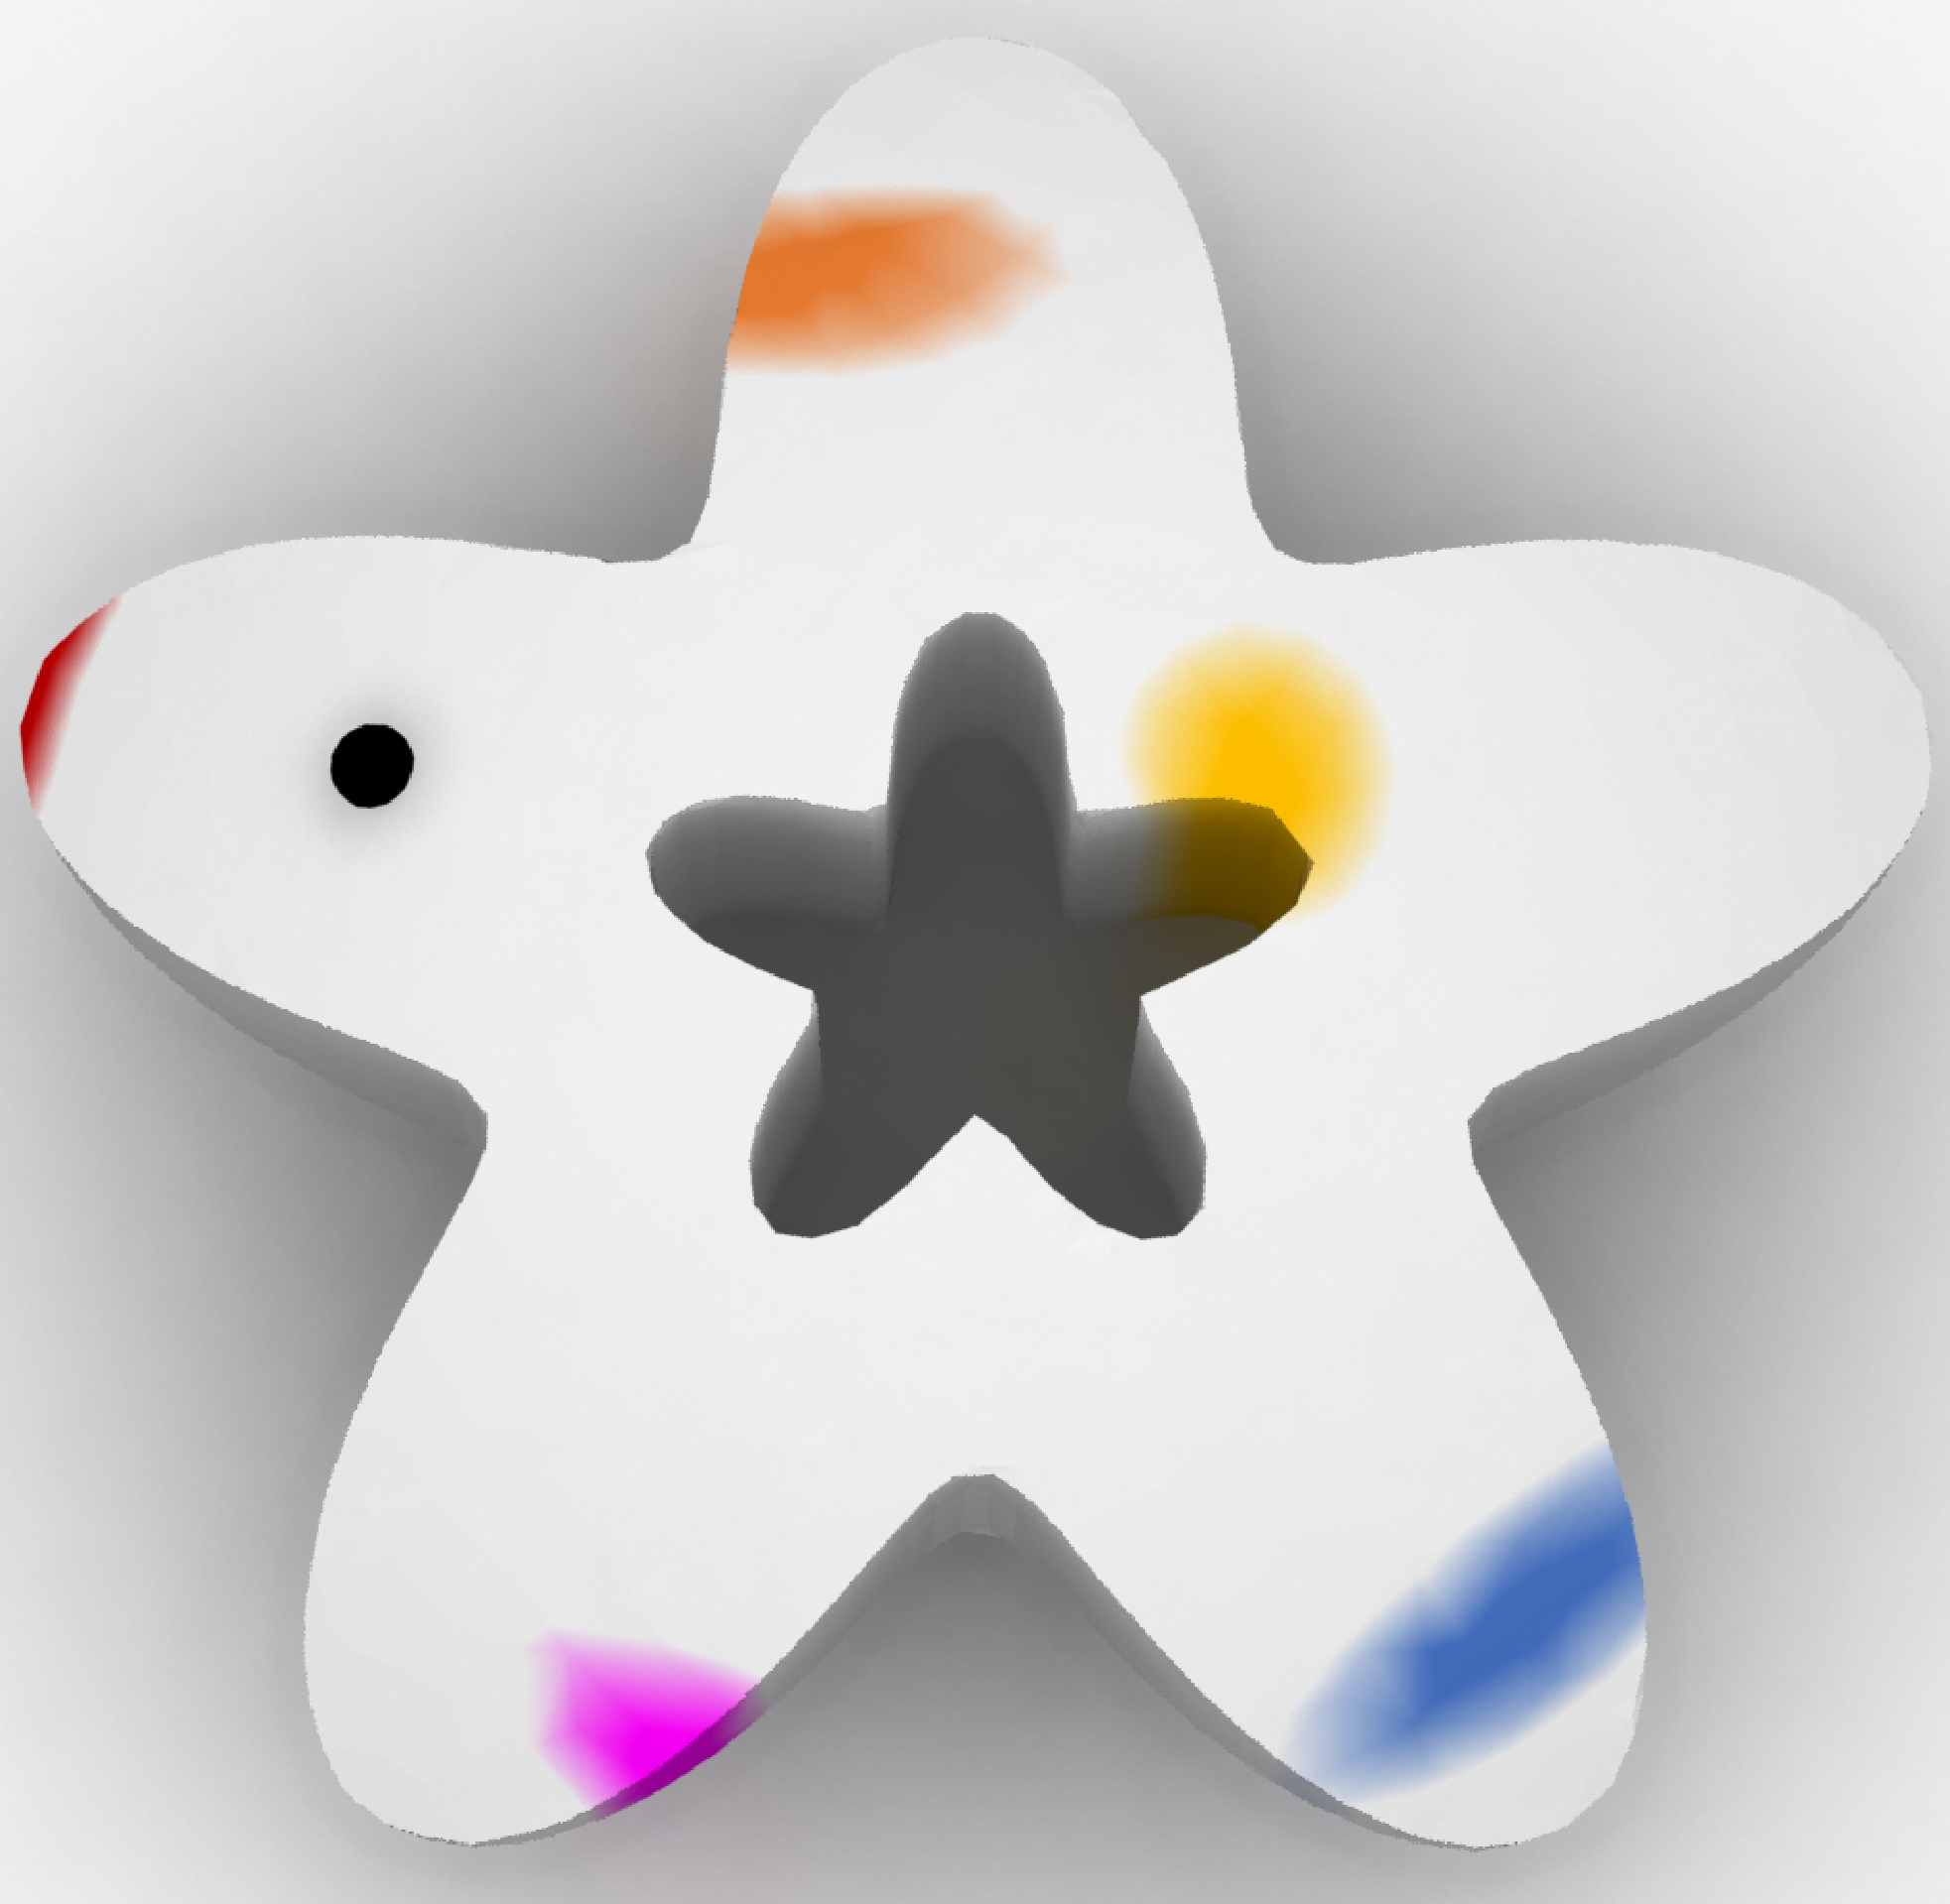
\includegraphics[height=.12\linewidth]{figures/interactive/point_map_target_cropped.pdf}&
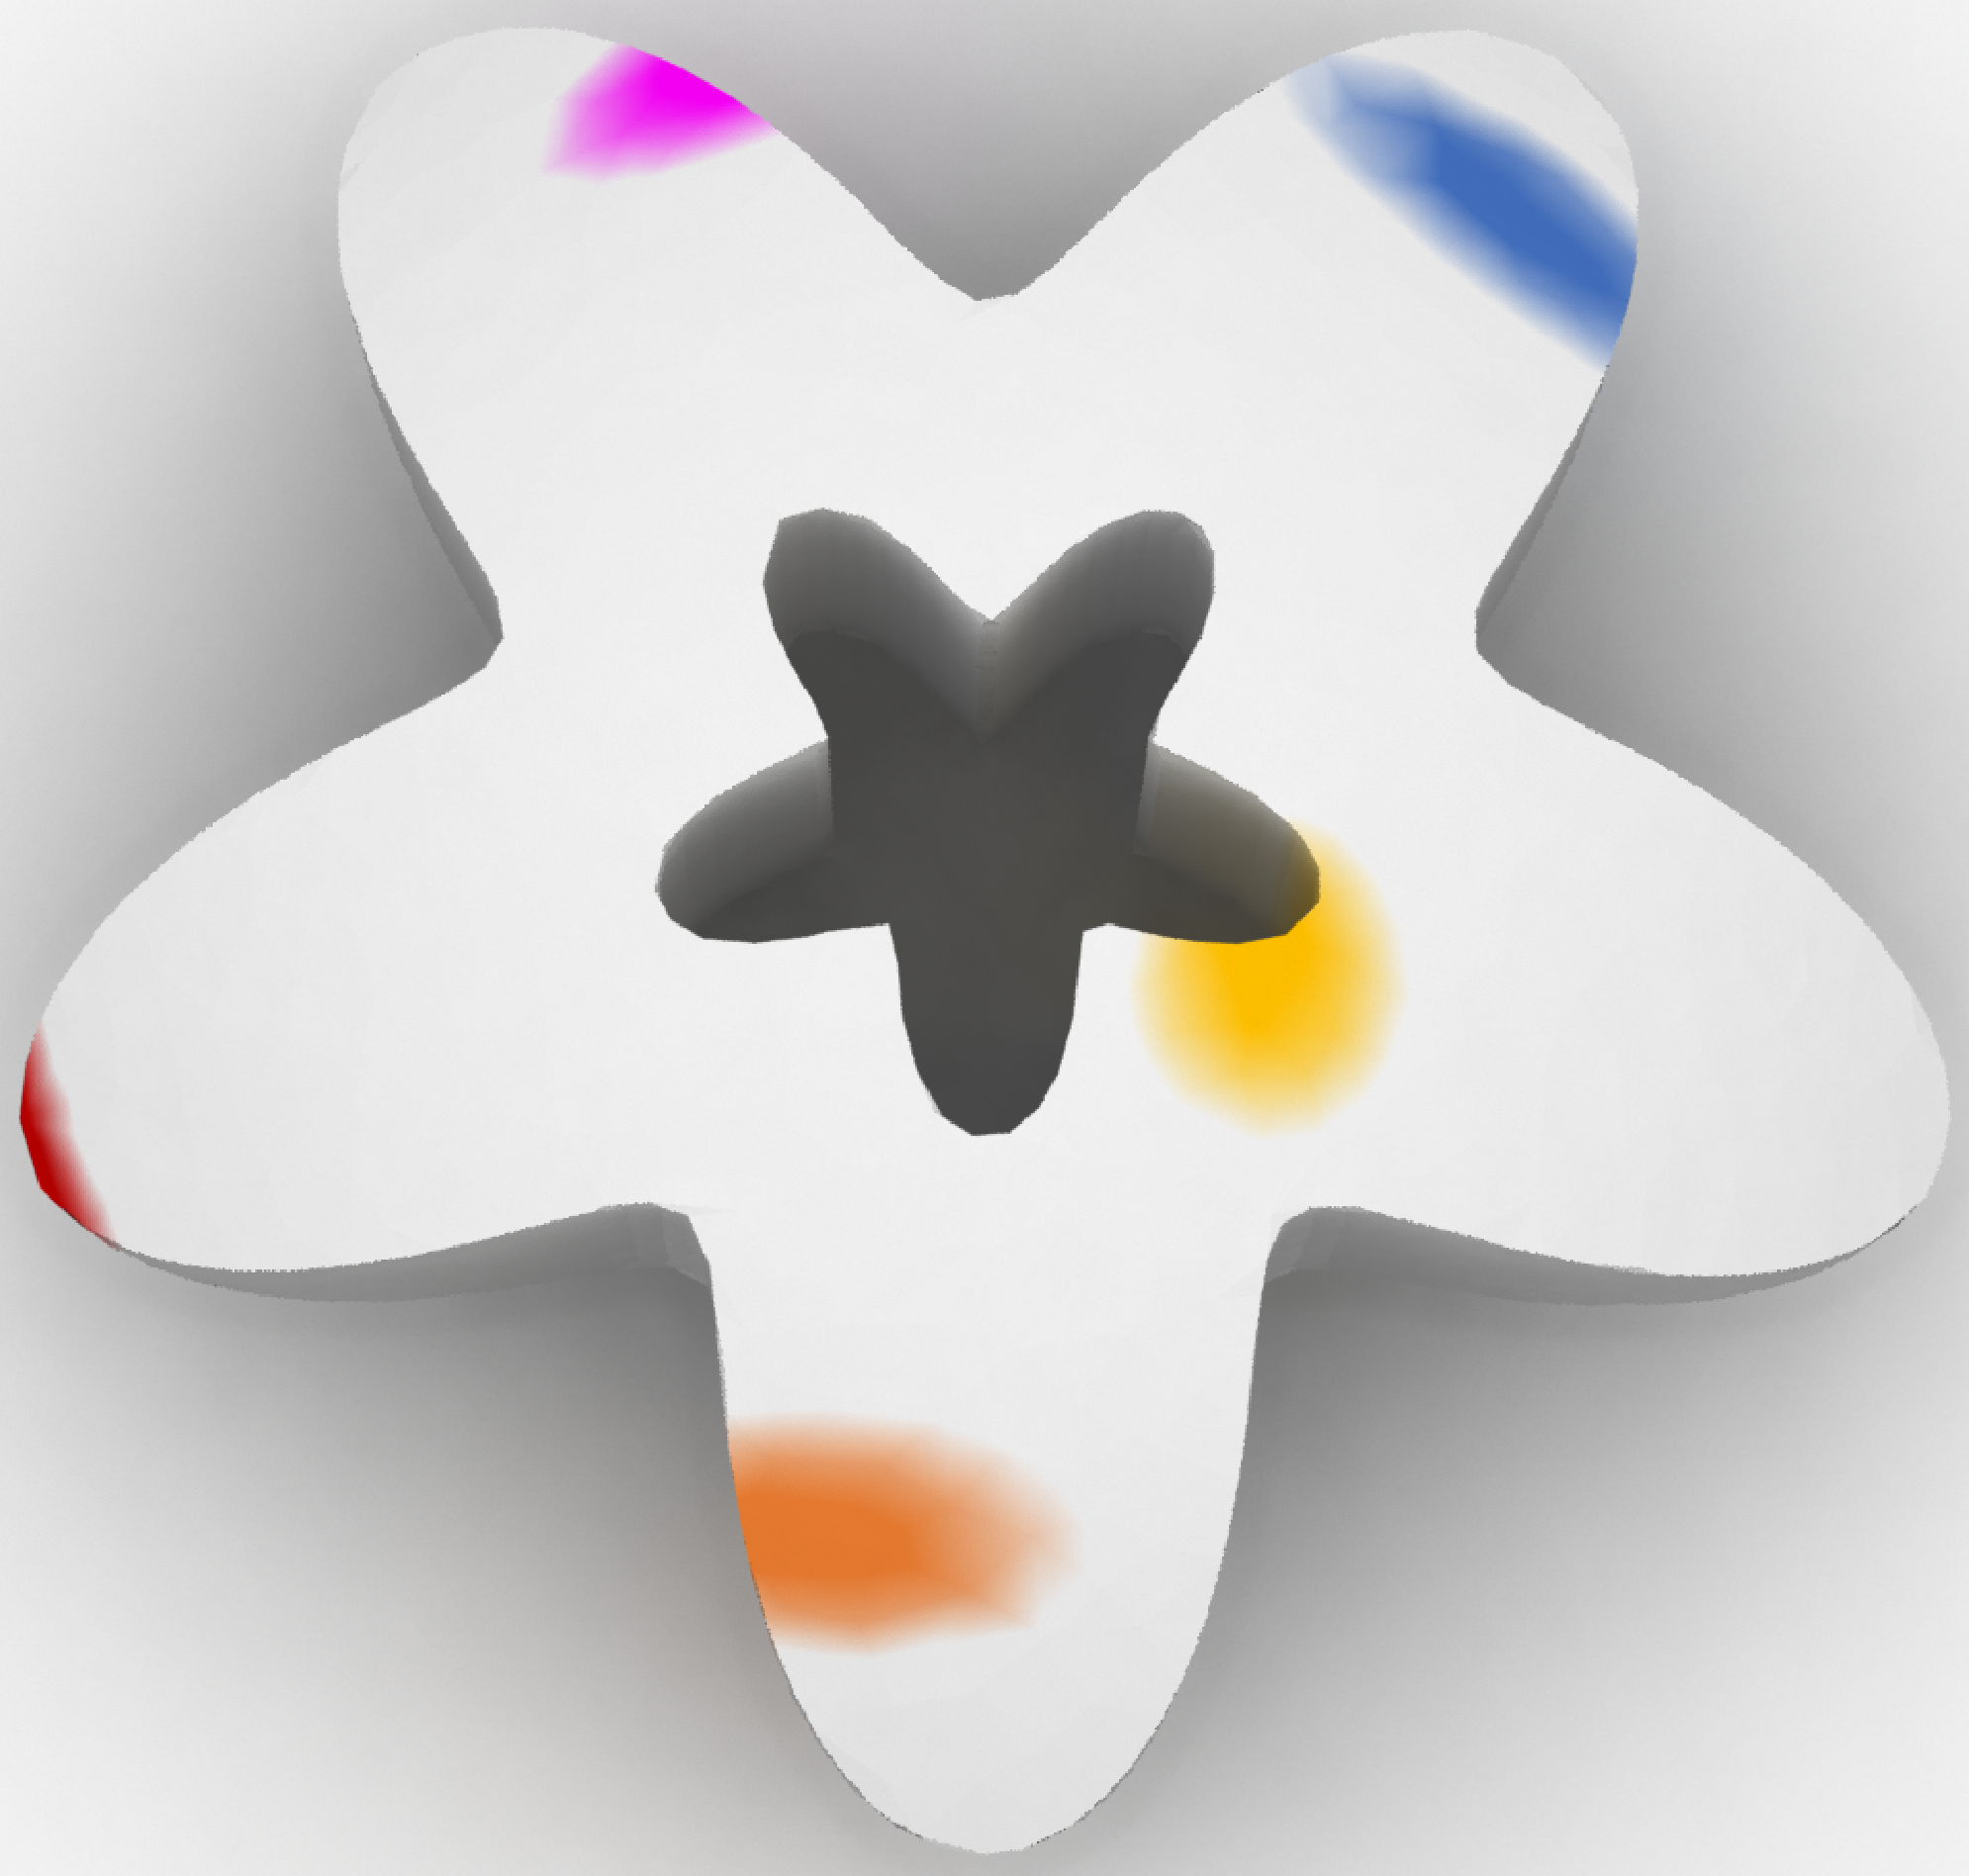
\includegraphics[height=.12\linewidth]{figures/interactive/point_map_target_flip_cropped.pdf}&
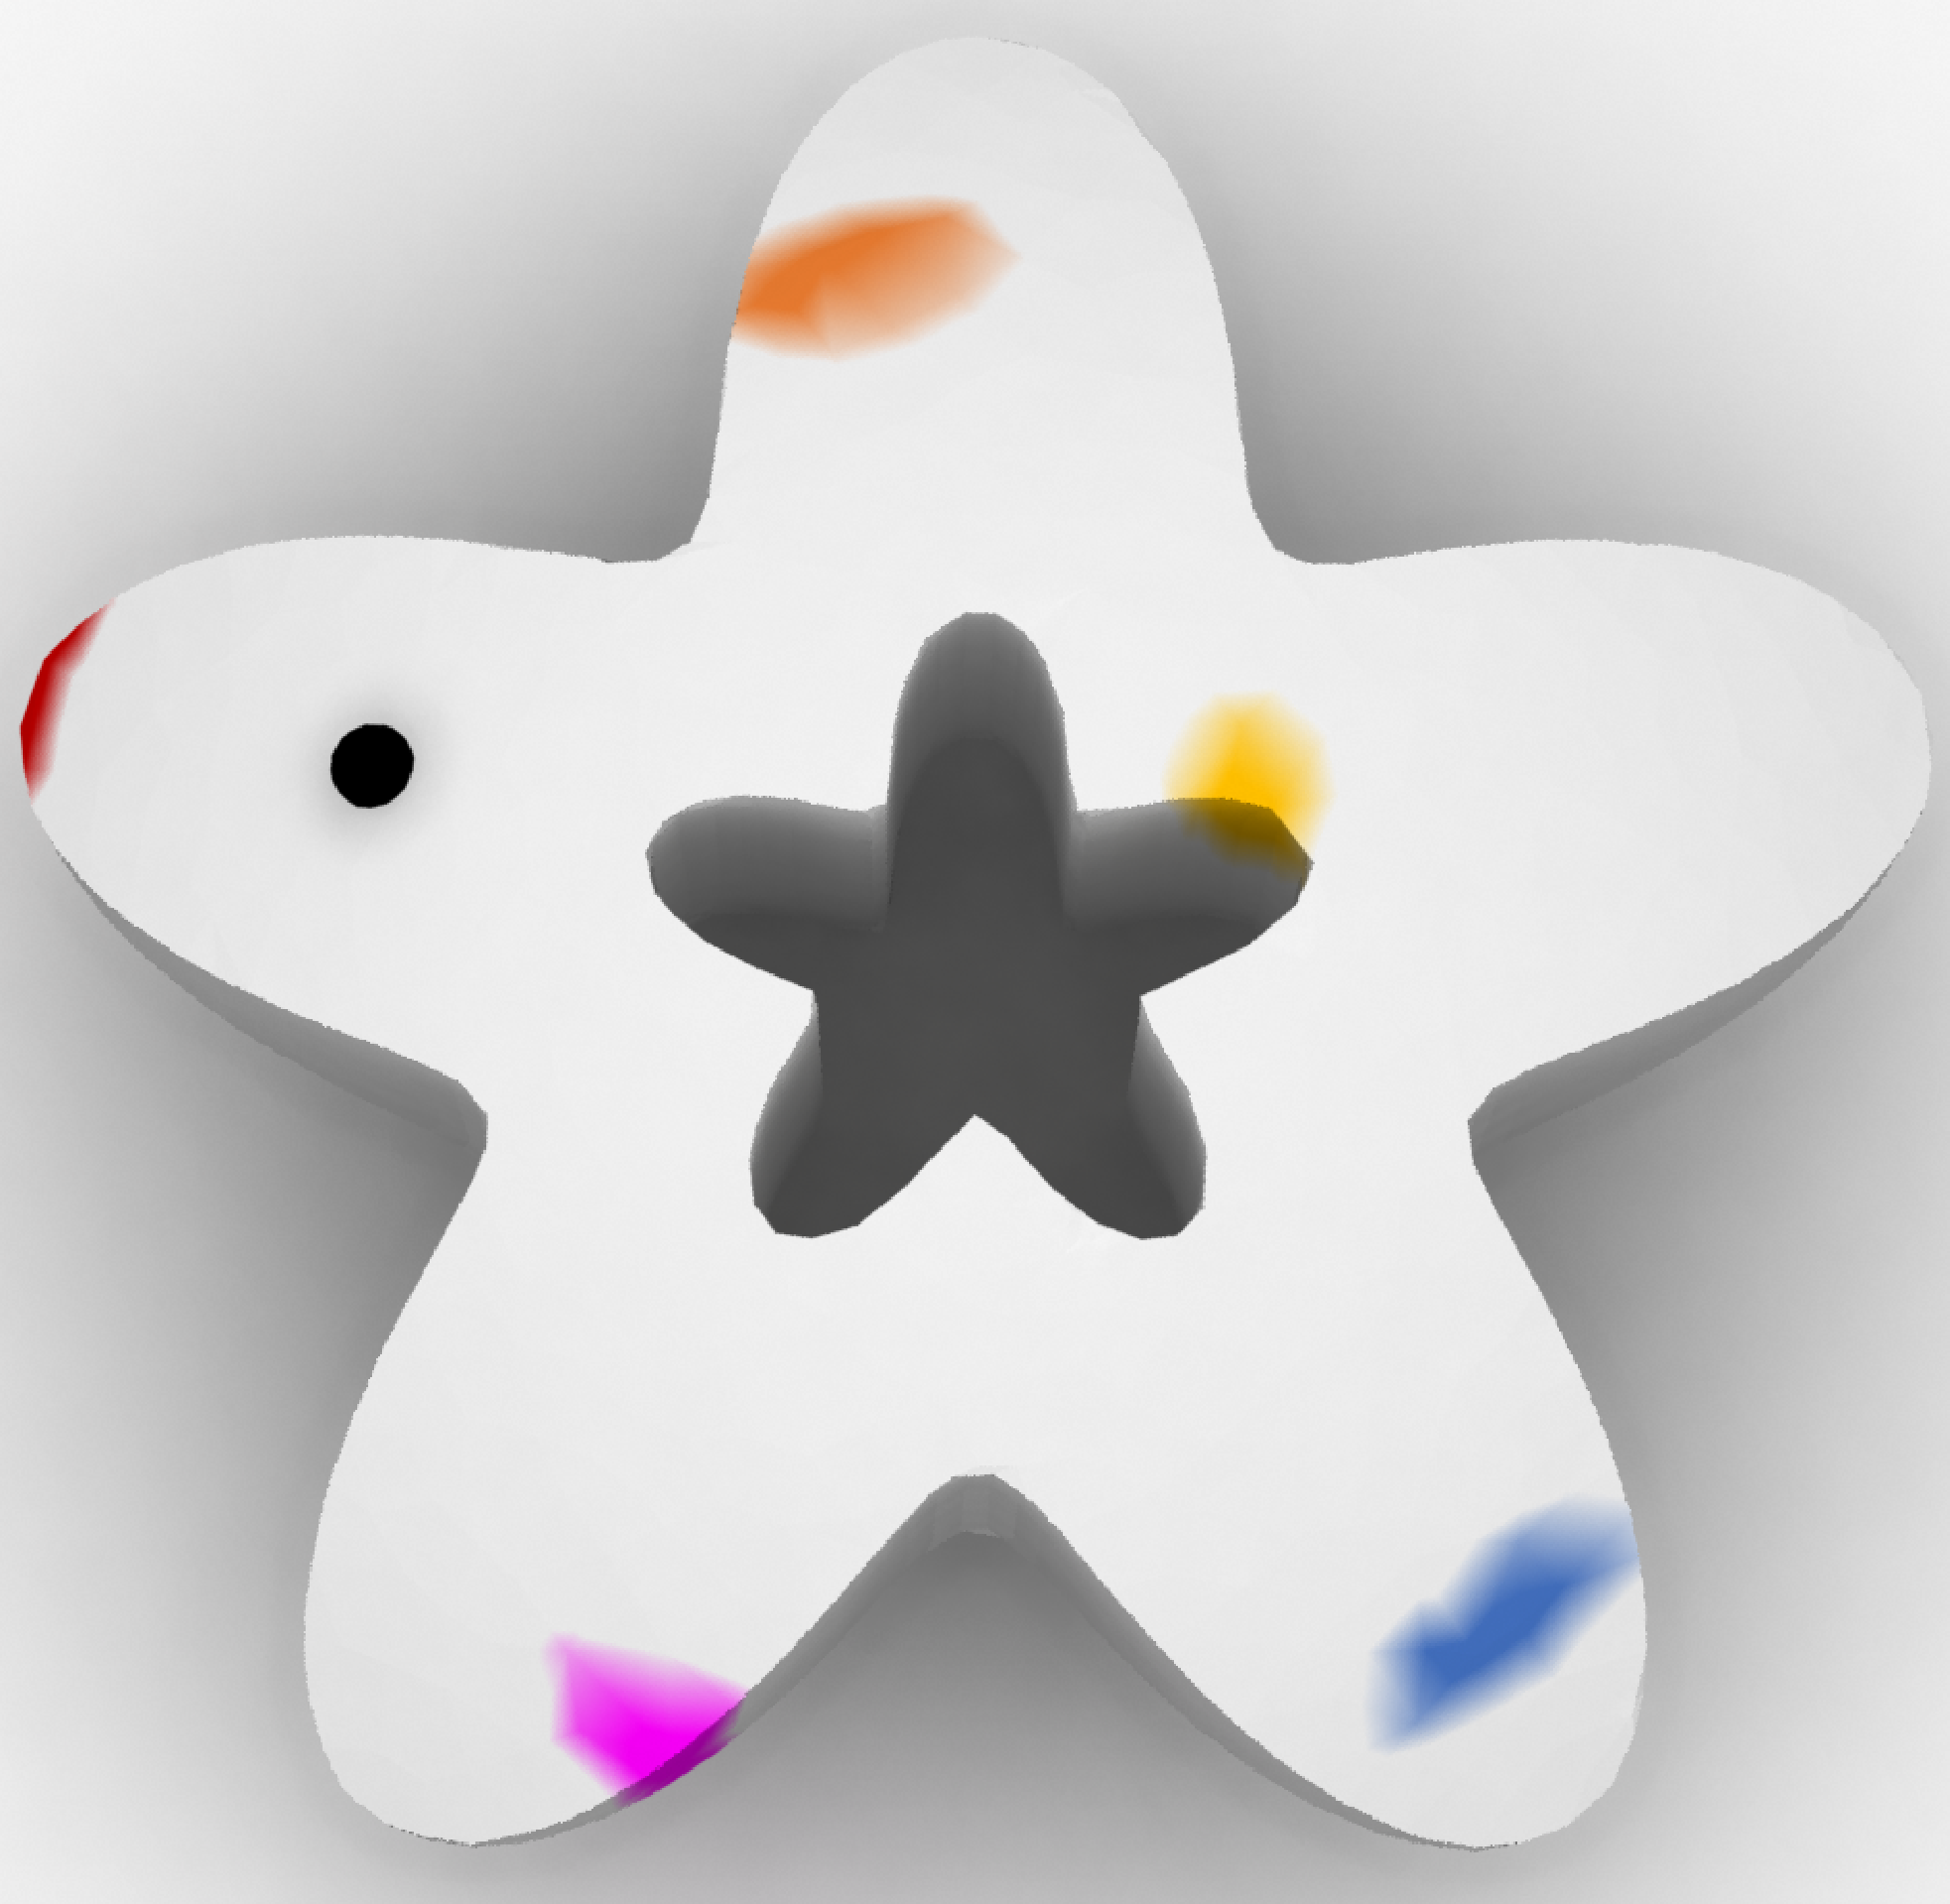
\includegraphics[height=.12\linewidth]{figures/interactive/reflection_map_target_cropped.pdf}&
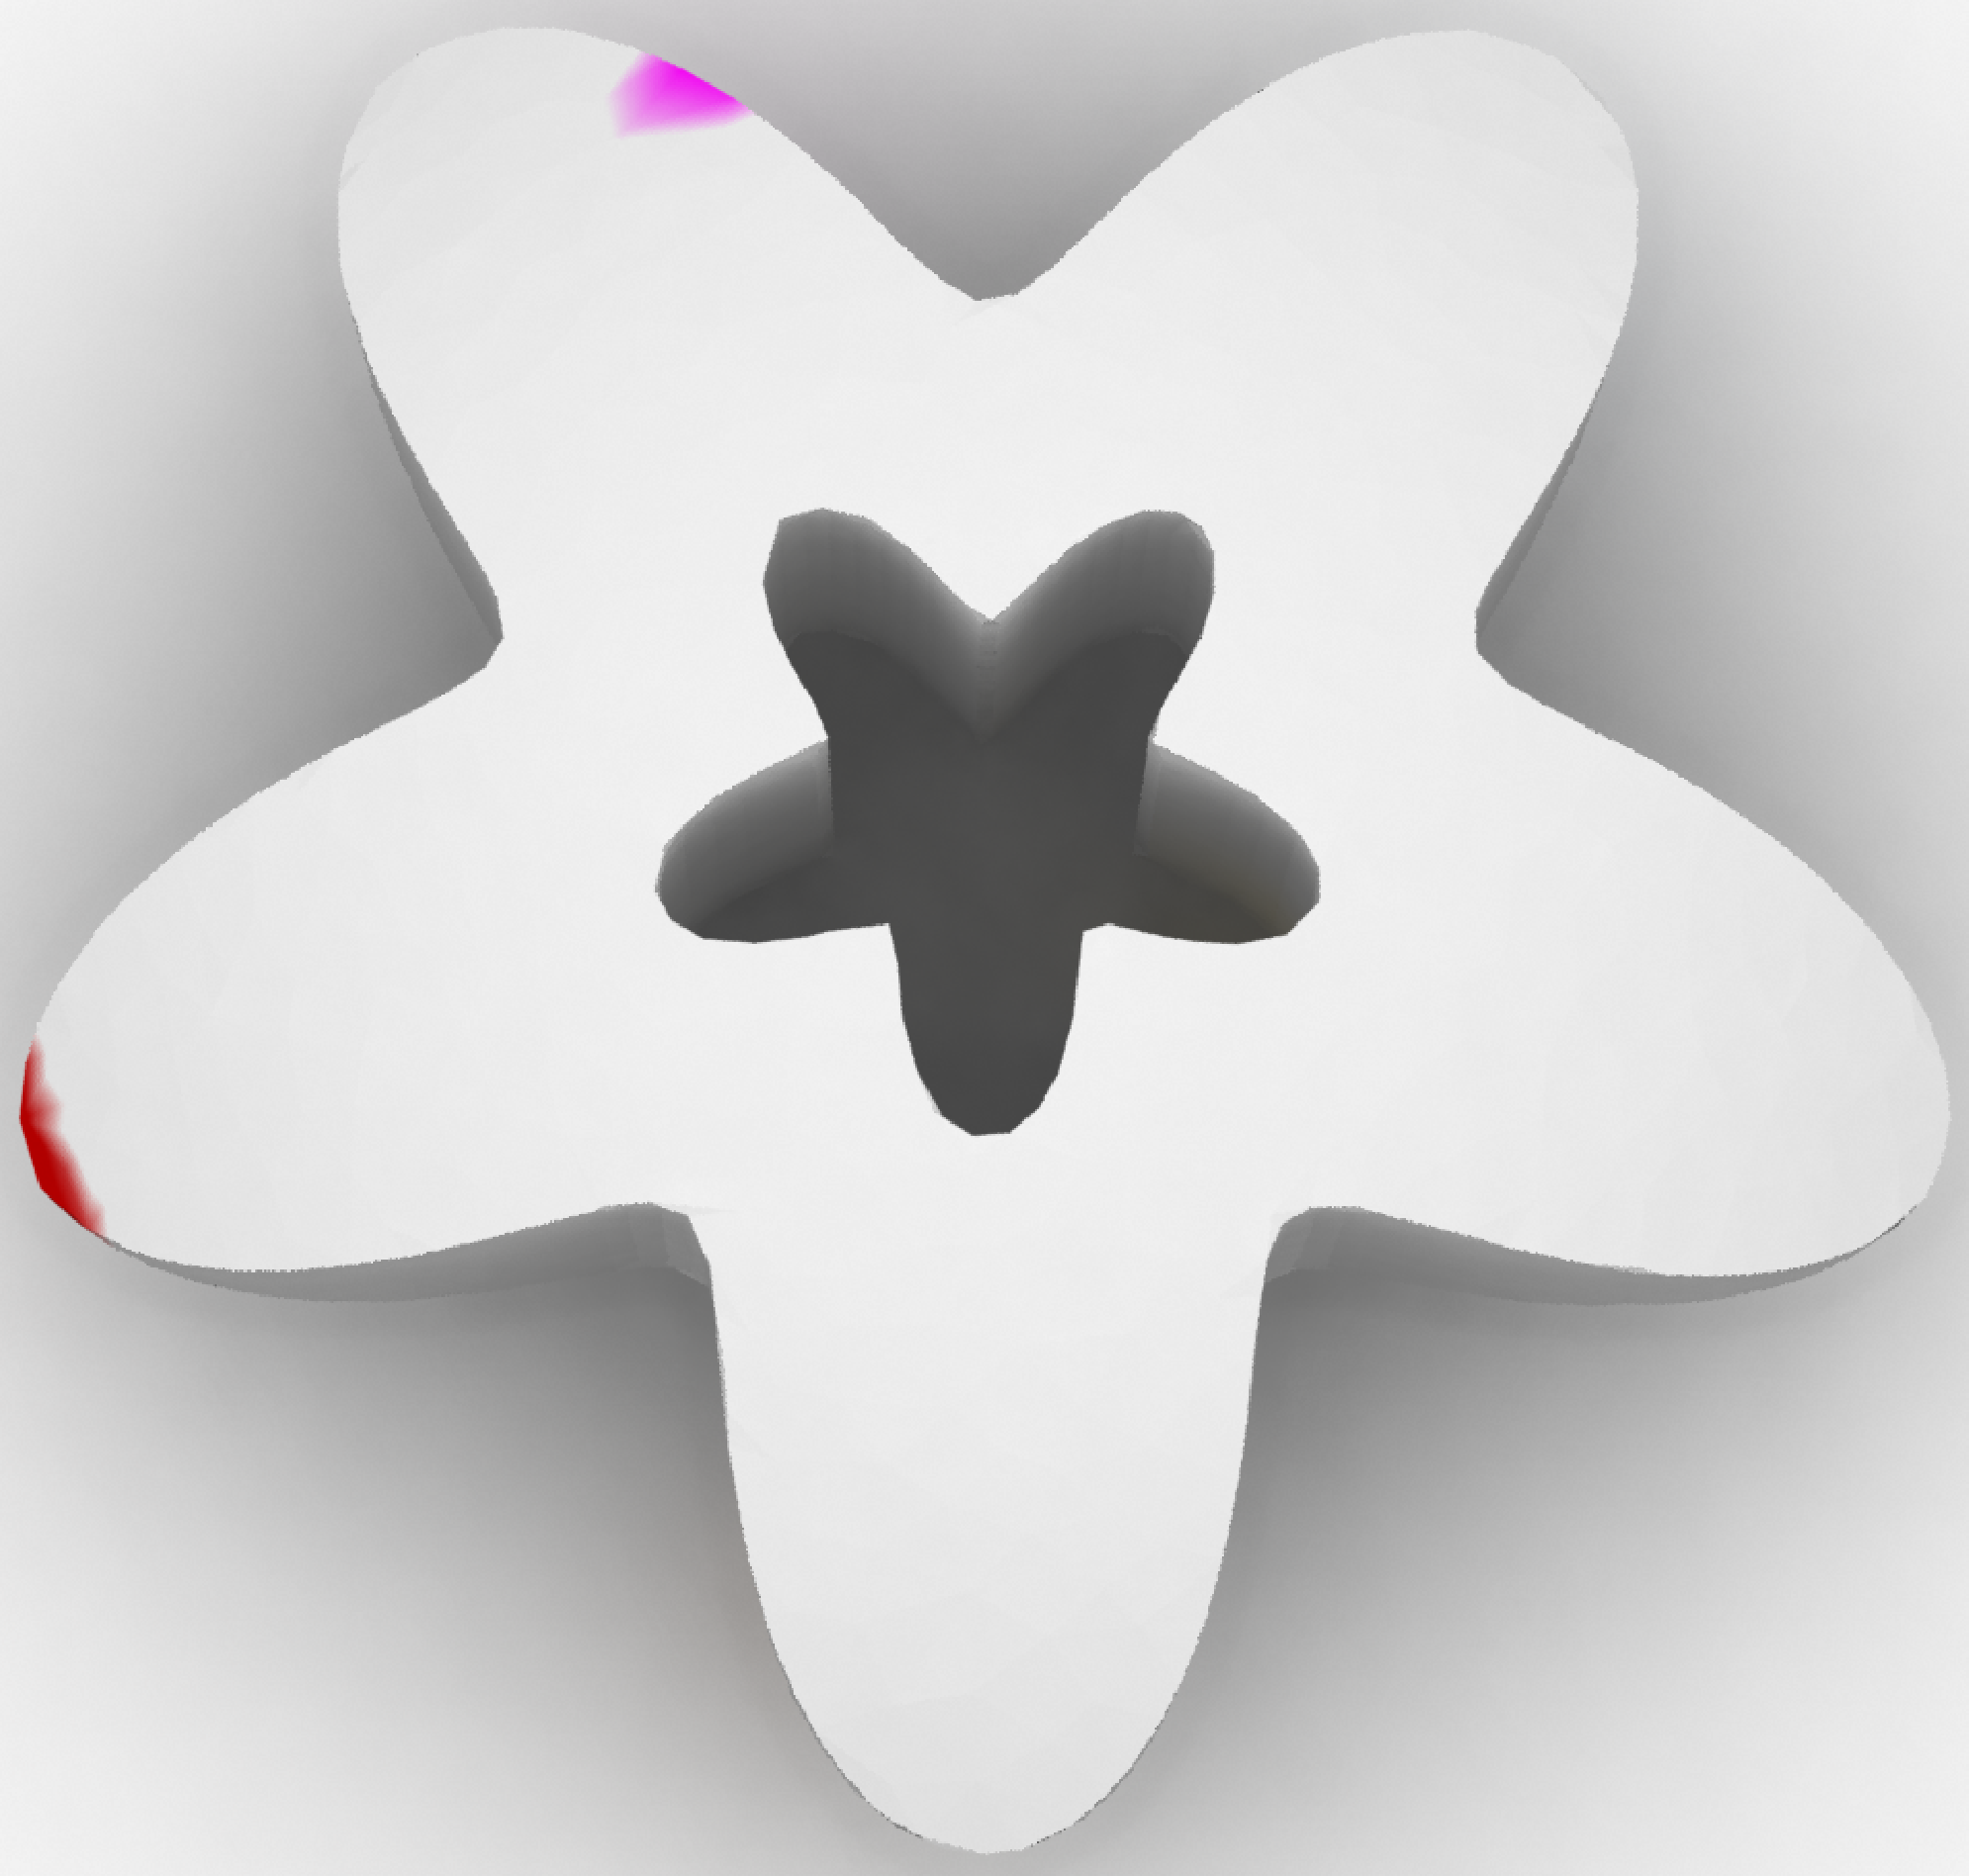
\includegraphics[height=.12\linewidth]{figures/interactive/reflection_map_target_flip_cropped.pdf}\\
Source  & 
\multicolumn{2}{c}{Unconstrained (black point image)}&
\multicolumn{2}{c}{Point constraint}&
\multicolumn{2}{c}{Point \& plane constraints}\\
& \multicolumn{2}{c}{\small $\alpha\!=\!8\!\times\!10^{-3}$}
& \multicolumn{2}{c}{\small $\alpha\!=\!5\!\times\!10^{-4}$}
& \multicolumn{2}{c}{\small $\alpha\!=\!2.5\!\times\!10^{-4}$}
\end{tabular}\vspace{-.125in}
\caption{Steps in supervised map design user session, outlined in \S\ref{sec:supervised_matching}.\vspace{-.15in}}\label{fig:supervised_map}
\end{figure*}
Figure~\ref{fig:supervised_map} illustrates a prototype ``user session'' in interactive map design.  Initially, we optimize with high regularization and no constraints, yielding a superposition of symmetric maps.  The user is prompted with the highest-entropy row (leftmost target; source point marked in black) and inputs a ground truth match, marked in black in the remaining target images.  The map is recomputed with a lower regularizer and the ground truth match in $\bS$, disambiguating the rotational symmetry (center target).  \GWa is still unable to disambiguate the top-bottom reflectional symmetry, so the user further constrains the upper half of the source to map to the upper half of the target by using $\S$ to zero out undesired matches.  With this additional change and after decreasing regularization, the algorithm produces a near point-to-point map (rightmost target).  Each map update takes a few seconds.

\subsection{Weighted Distance Matrix}\label{sec:weighted_mtx}

\begin{figure}[t]\centering
\includegraphics[width=\linewidth]{figures/image_grid/weightedImageLayout.pdf}
\caption{Mapping a set of 185 images onto a two shapes while preserving color similarity. \small{(Images from Flickr public domain collection.)}\vspace{-.15in}}\label{fig:weighted_images}
\end{figure}

In some scenarios, only distances in a particular range are relevant to matching, e.g.\ keeping certain points close to one another while pushing others far apart.  In other contexts, distance values may be known with varying confidence.

More generally, suppose in addition to distance matrices $\D_0\in\R_+^{n_0\times n_0}$ and $\D\in\R_+^{n\times n}$ we are given symmetric weight matrices $\bW_0\in\R_+^{n_0\times n_0}$ and $\bW\in\R_+^{n\times n}$.  We could solve a \emph{weighted} version of the \GWa matching problem~\eqref{eq:GW2} that prioritizes maps preserving distances corresponding to large $\bW$ values:
\begin{equation}\label{eq:weighted_gw}
\min_{\G\in\bM} \sum_{ijk\ell} (\D_{0ij}\!-\!\D_{k\ell})^2\G\!_{ik}\G\!_{j\ell}\!\bW_{0ij}\!\bW_{j\ell}\bmu_{0i}\bmu_{0j}\bmu_k\bmu_\ell.
\end{equation}
For instance, $(\bW_0,\bW)$ might contain confidence values expressing the quality of the entries of $(\D_0,\D)$.  Or, $\bW_0,\bW$ could take values in $\{\varepsilon,1\}$ reducing the weight of distances that are unknown or do not need to be preserved by $\G$.

Following the same simplifications as \S\ref{sec:gw_matching}, we can optimize this objective by minimizing $\langle\G,\bL_\bW(\G)\rangle,$ where
\begin{align*}
\bL_\bW(\G)\eqdef&
\frac{1}{2}[\D_0^{\wedge2}\otimes \bW_0]\diag{\bmu_0}\G\diag{\bmu}\bW
\\&- [\D_0\otimes \bW_0]\diag{\bmu_0}\G\diag{\bmu}[\D\otimes \bW]
\\ &+\frac{1}{2} \bW_0\diag{\bmu_0}\G\diag{\bmu} [\D^{\wedge2}\otimes \bW]
\end{align*}
The remainder of the derivation in \S\ref{sec:gw_matching} remains unchanged, and hence we can optimize~\eqref{eq:weighted_gw} using a small modification of Algorithm~\ref{alg:gw} corresponding to the new update rule
$$
\G^{(k\!+\!1)}_\bW\!\gets\!\argmin_{\G\in\bM}%(\bmu_0,\bmu)}
%
\KL\!\left(\!\G\!
\left|\!
\left[\!\exp\!\left(\!-\frac{\bL_\bW(\G^{(k)}_\bW\!)}{\alpha}\!\right)\!\right]^{\wedge\eta}\!\otimes\!\left[\G^{(k)}_\bW\right]^{\wedge(1-\eta)}\right.
\!\right)\!.
$$
In practice, giving $\bW$ exactly zero entries can cause numerical problems during Sinkhorn rescaling, so we bound it below by a small $\varepsilon>0$.%\suv{Hopefully zero weights don't break the KL-divergence stuff, e.g. iteration (7)}

Figure~\ref{fig:weighted_images} illustrates an application of this technique ($\alpha\!=\!3\!\times\!10^{-3},\eta\!=\!2.5\!\times\!10^{-2}$).  Here, we extend the image example from \S\ref{sec:experiments} to map images onto shapes on a shared grid.  We take $\bW_{ij}\!=\!1$ if $i$ and $j$ are in the same connected component and $\bW_{ij}\!=\!0$ otherwise; this objective does not enforce color continuity between the connected components.  As a result, the components exhibit different (but still smooth) color variations, e.g.\ the clusters of blue images on the two components are distant from each other.  Note the optimization decides which image appears in which cluster.


\subsection{Symmetry Detection}\label{sec:symmetry}

\cite{pauly2015} recently posed the question of whether optimal transportation can be used for symmetry analysis.  We outline one strategy here for dealing with symmetries intrinsic to the distance matrices $\D_0,\D$ leveraging the \emph{non}-convexity of the \GWa objective function.

Suppose Algorithm~\ref{alg:gw} yields a measure coupling $\G$ corresponding to a map $\source\mapsto\target$.  If the distance matrix $\D$ on $\target$ has a symmetry, then there exists a second coupling $\G'$ with a similar \GWa objective value encoding the symmetric map.  We optimize for this map by biasing the \GWa objective slightly against $\G$ in~\eqref{eq:reg_gw}:% for $\varepsilon\!>\!0$:
\begin{equation}\label{eq:symm_objective}
\f^{\mathrm{symm}}_\alpha(\G';\G)\eqdef\exp([\D_0\diag{\bmu_0}\G'\diag{\bmu}\D-\varepsilon \G]/\alpha).
\end{equation}
Now, the symmetric map should have a slightly lower objective value than $\G$, which we can compute using the same algorithm.

\setlength{\columnsep}{2pt}
\begin{wrapfigure}[9]{r}{0.23\textwidth}\centering
\vspace{-.2in}
\begin{tabular}{c@{}c@{}c}
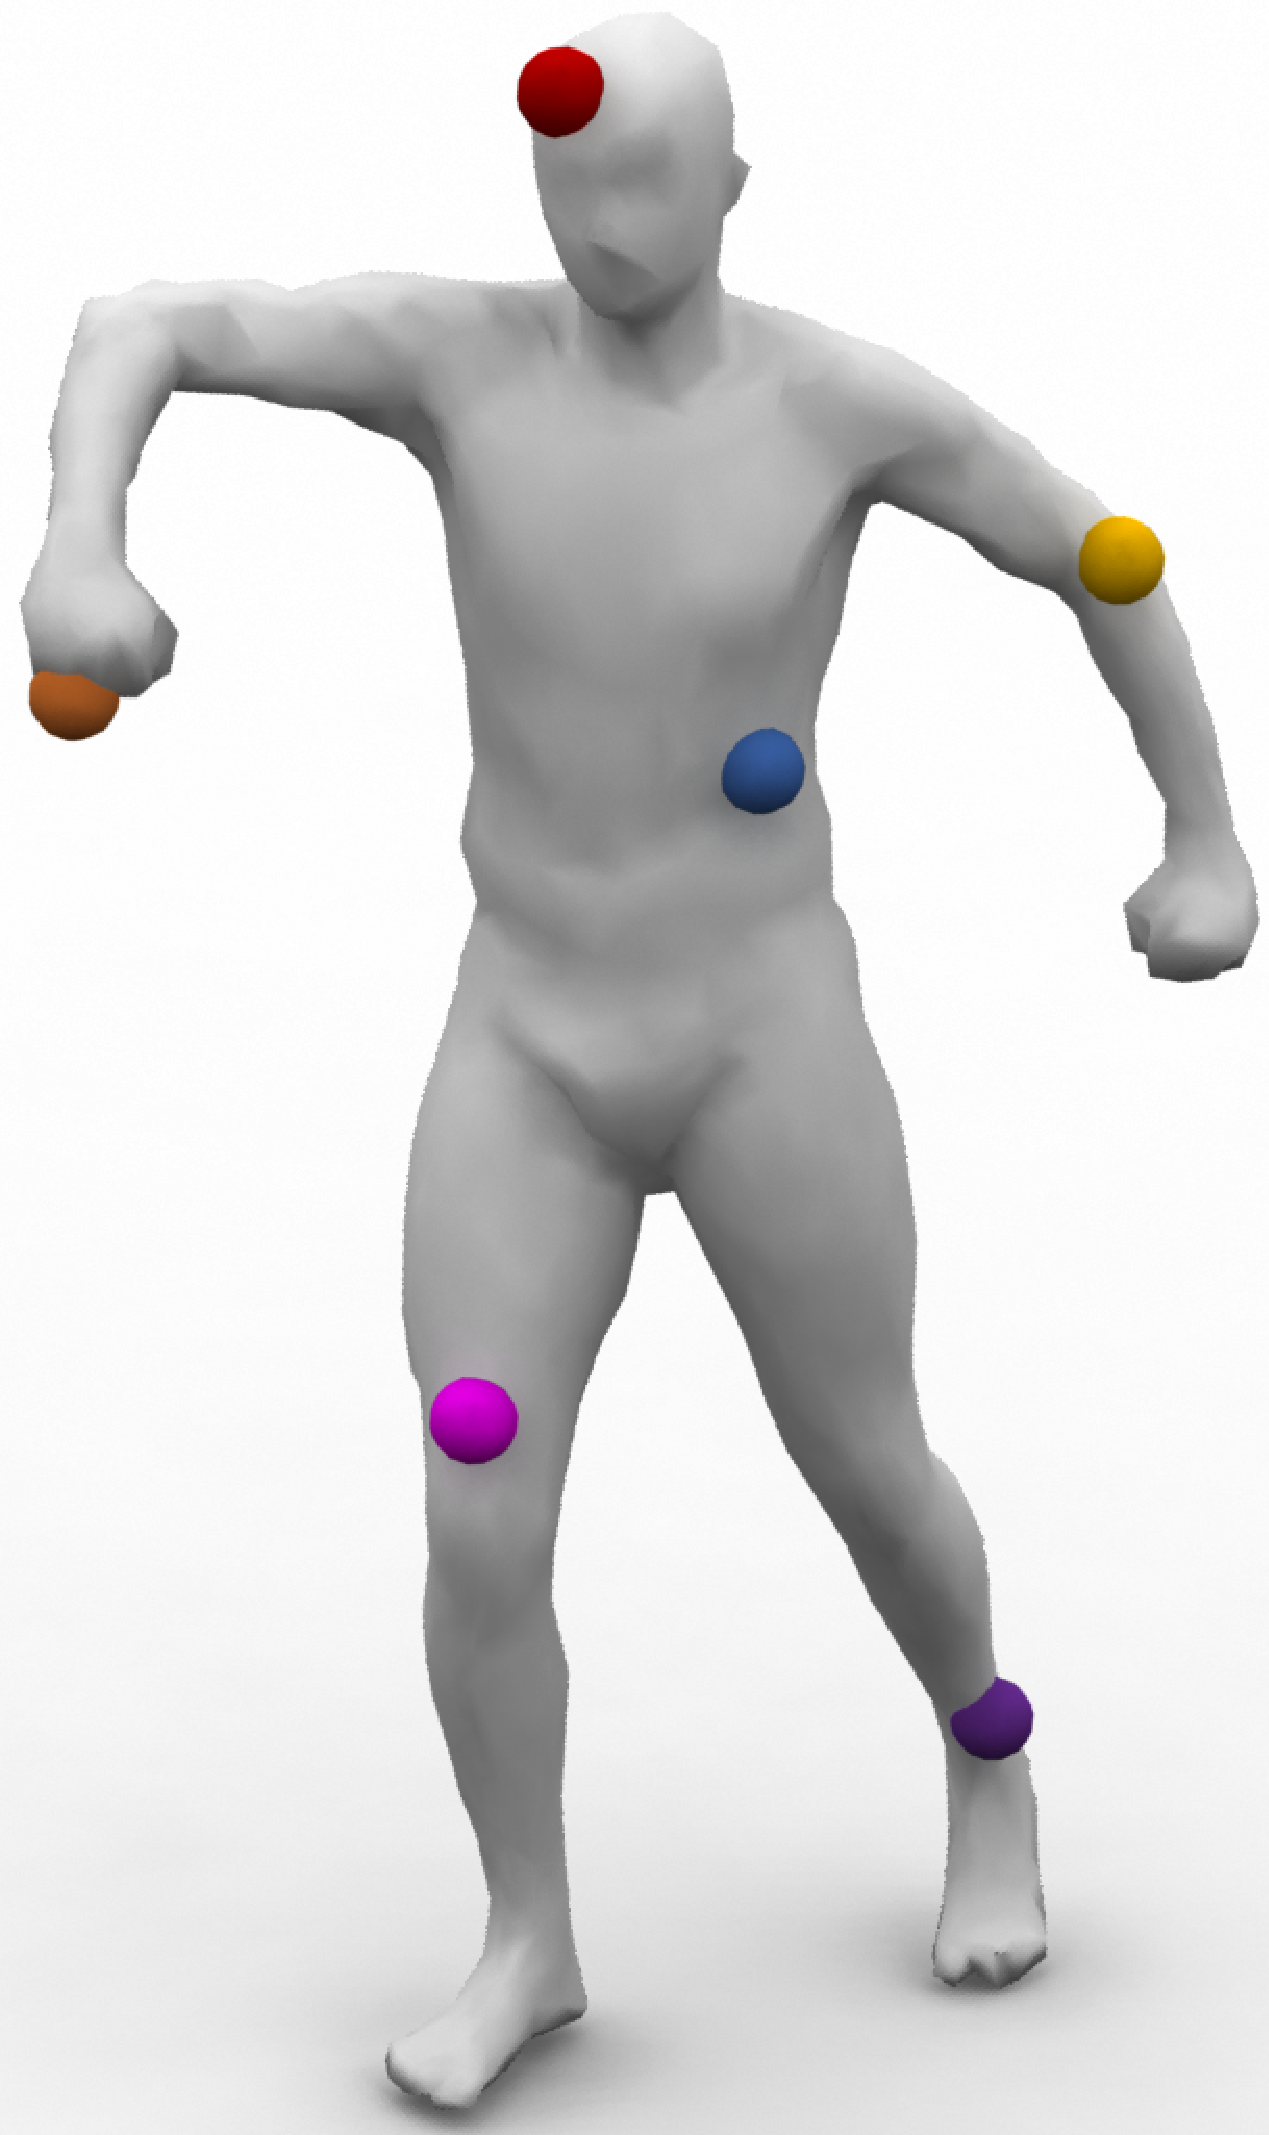
\includegraphics[height=.6\linewidth]{figures/symmetry/source_human.pdf}&
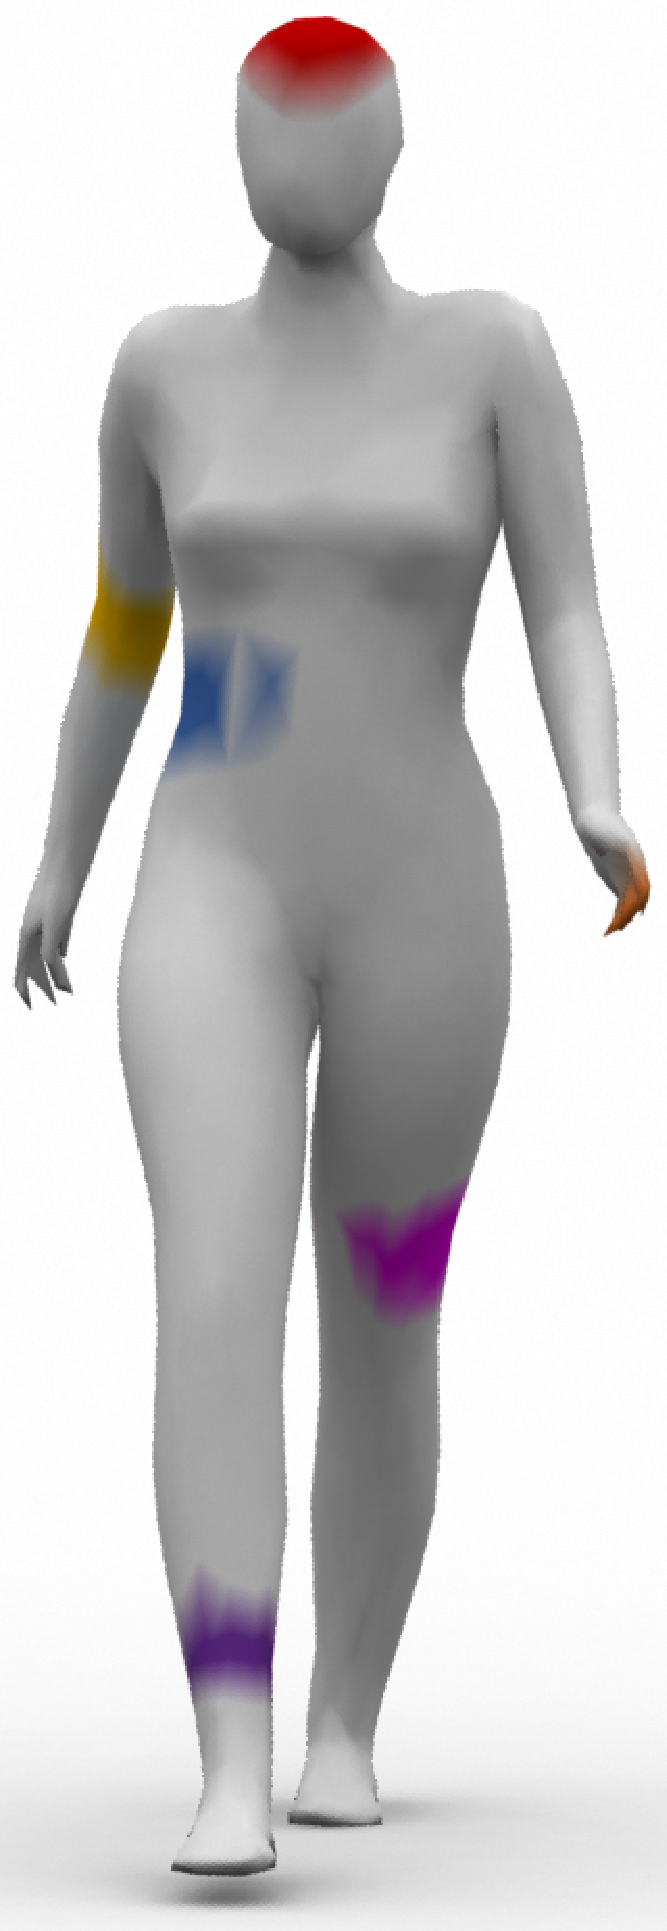
\includegraphics[height=.6\linewidth]{figures/symmetry/target_symmetric_humans_orig_cropped.pdf}&
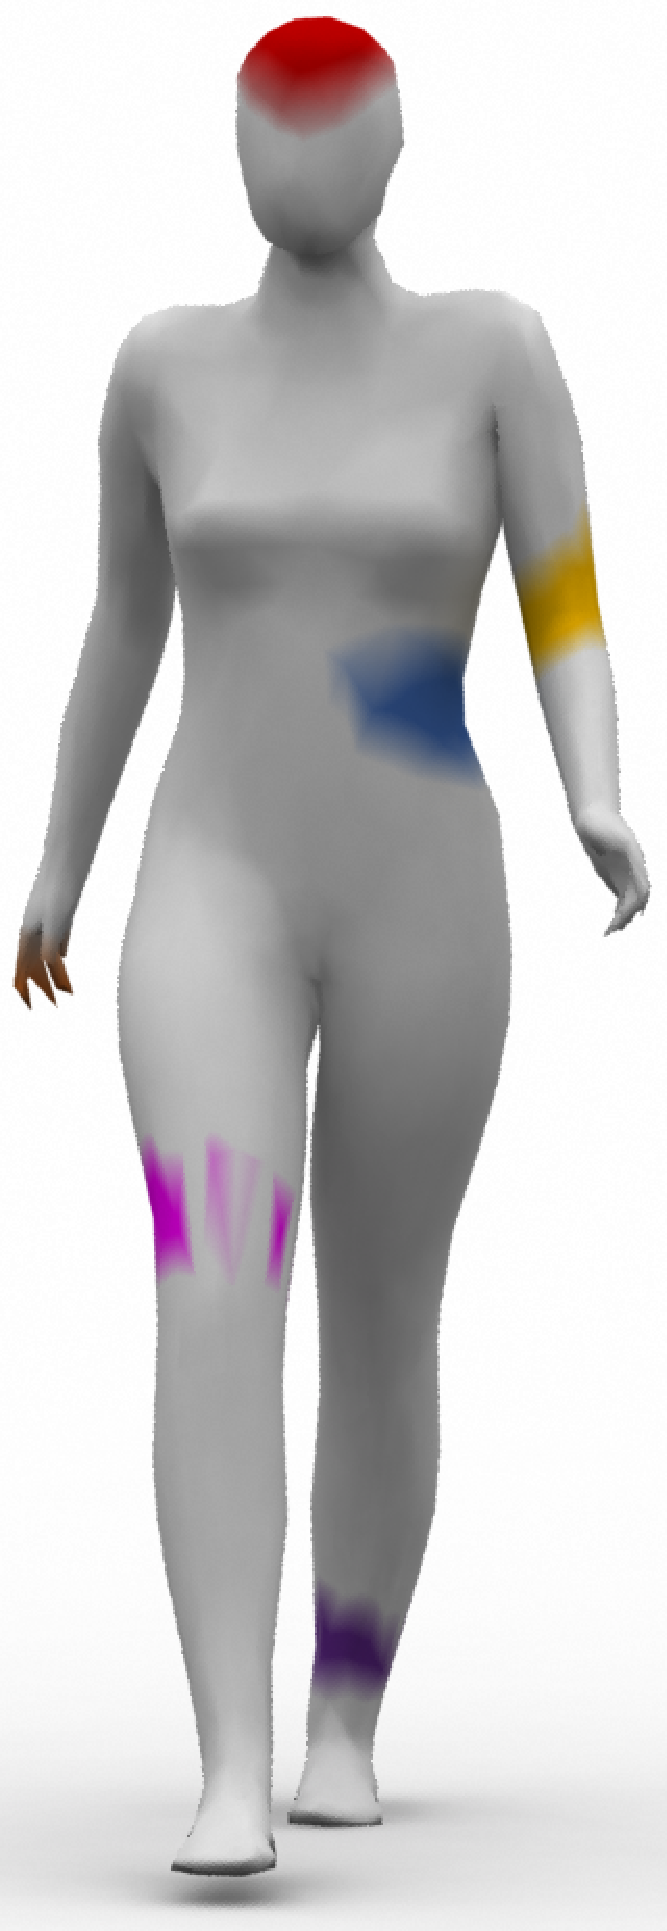
\includegraphics[height=.6\linewidth]{figures/symmetry/target_symmetric_humans_cropped.pdf}\\
$\source$ & $\G$ & $\G'$
\end{tabular}
\vspace{-.15in}
\caption{Symmetric maps.}\label{fig:symmetry}
\end{wrapfigure}
Figure~\ref{fig:symmetry} illustrates an example of symmetric map computation.  Algorithm~\ref{alg:gw} yielded the left-right reversing map between the meshes of humans (same as Figure~\ref{fig:more_maps}), which is equally optimal to the orientation-preserving map.  Fixing this map as $\G$ and optimizing for $\G'$ using~\eqref{eq:symm_objective} ($\varepsilon\!=\!10^{-6}$) yields the orientation-preserving map as desired.

\setlength{\columnsep}{2pt}
\begin{wrapfigure}[9]{r}{0.23\textwidth}\centering
\vspace{-.2in}
\begin{tabular}{c@{}c}
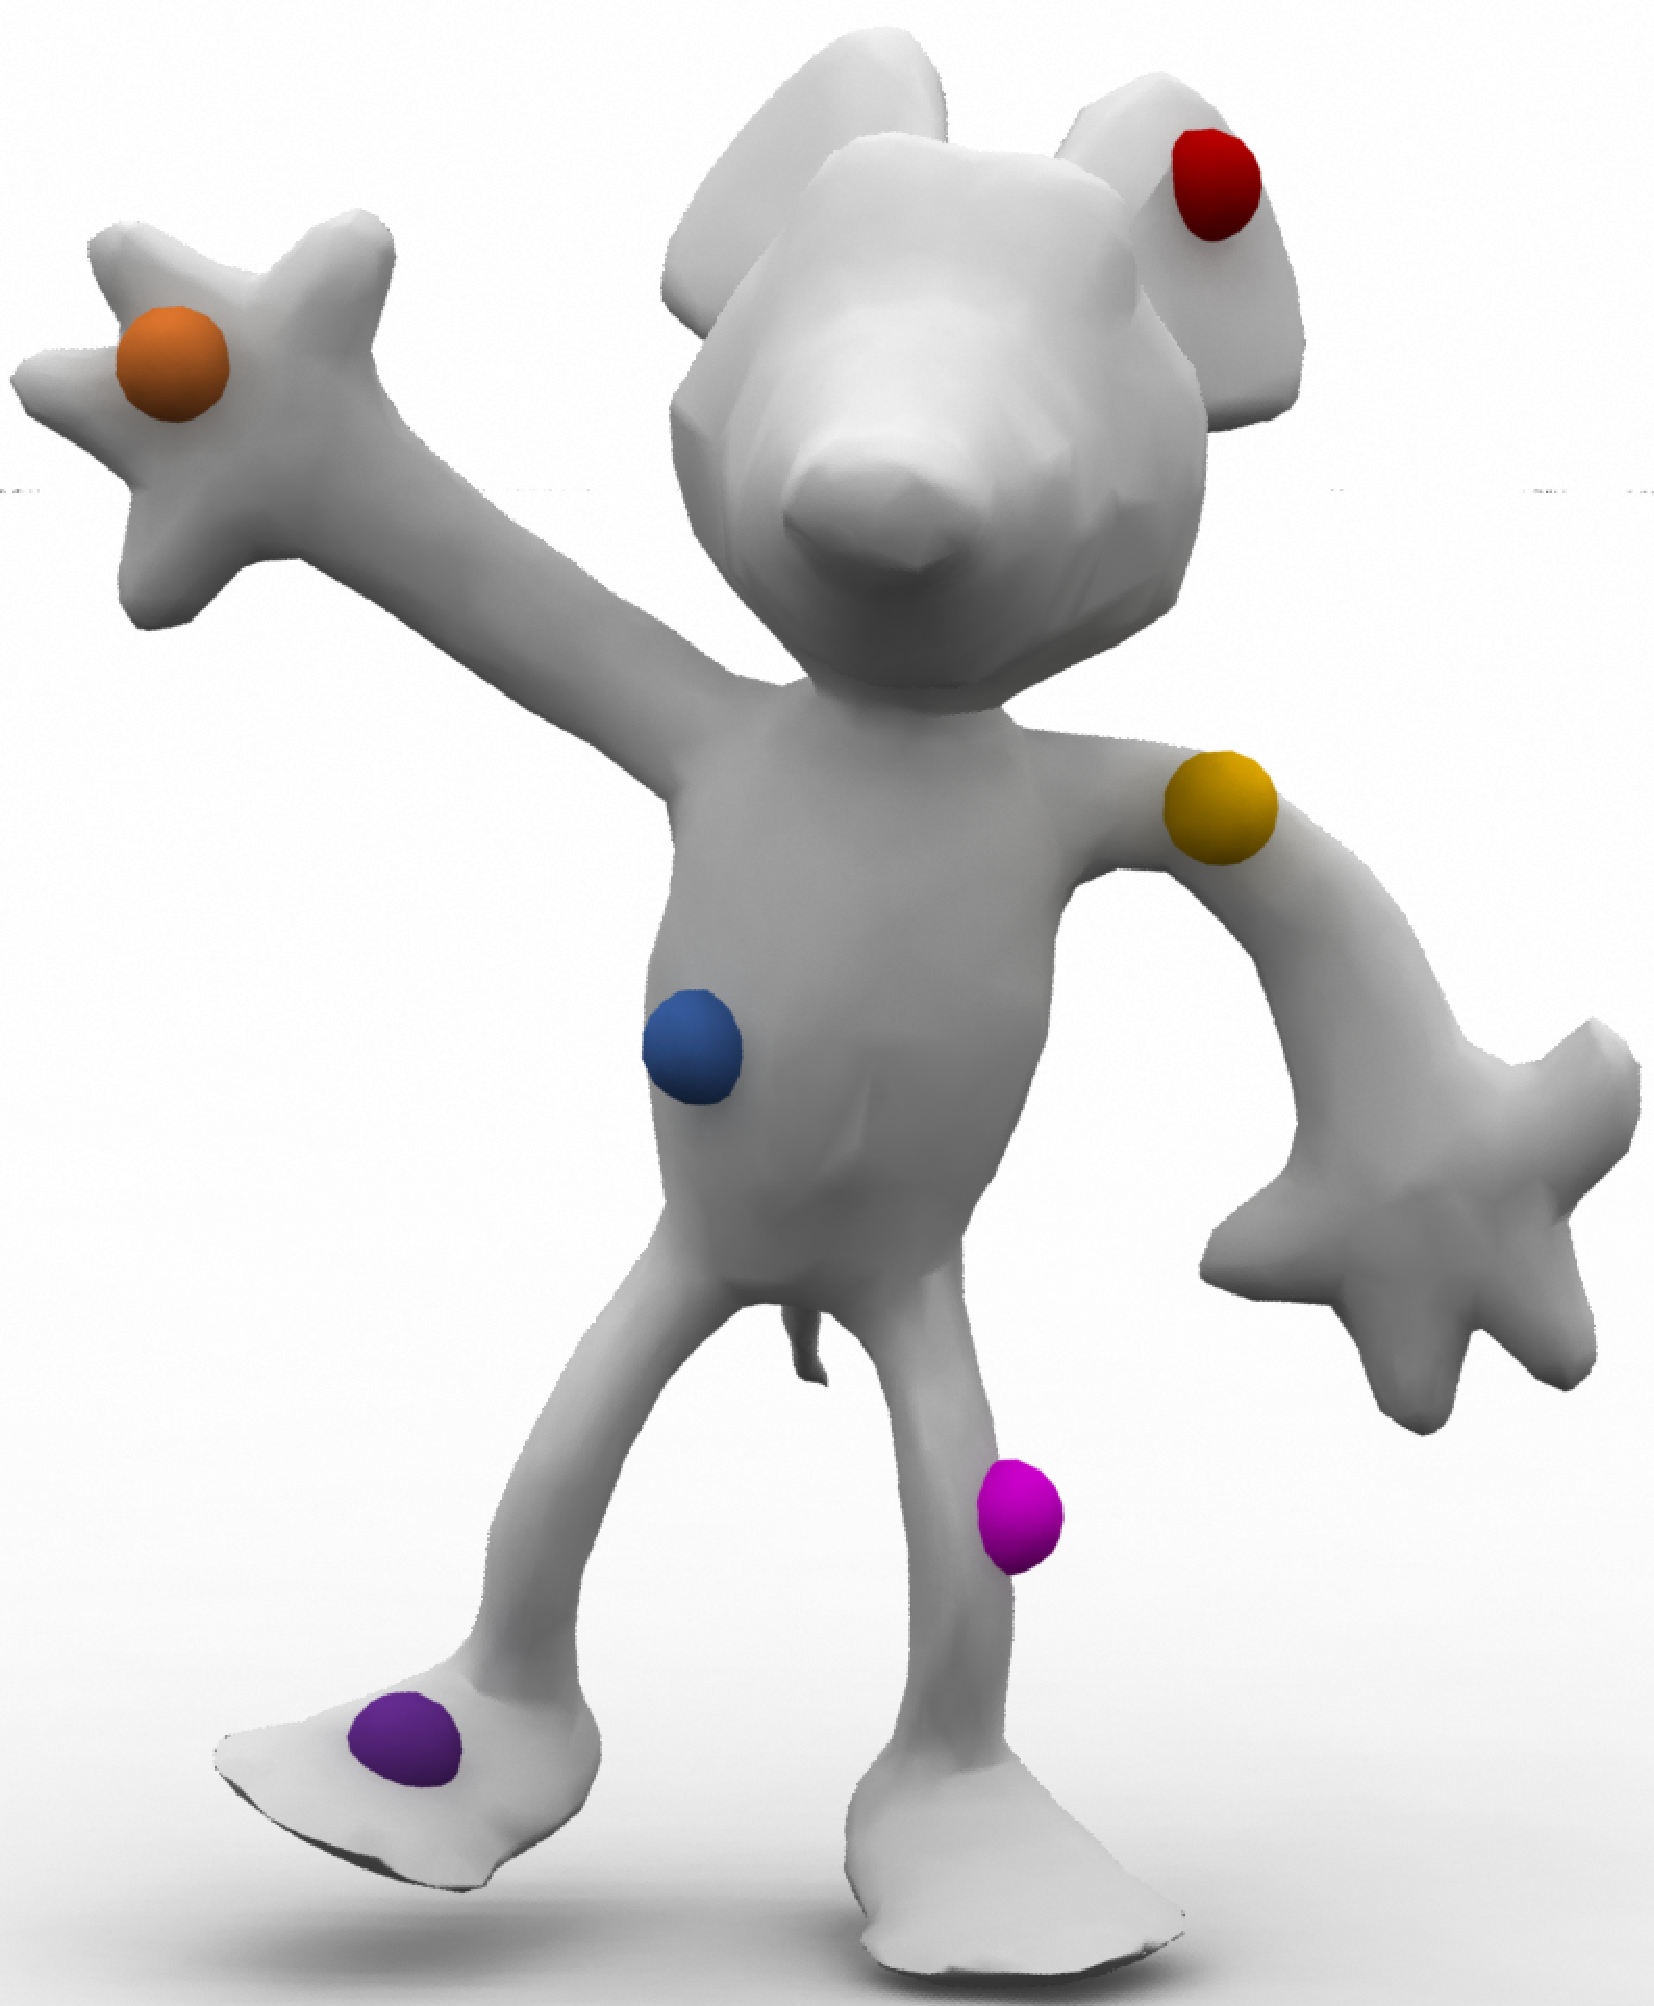
\includegraphics[height=.6\linewidth]{figures/symmetry/source_symmetric_mouse_cropped.pdf}&
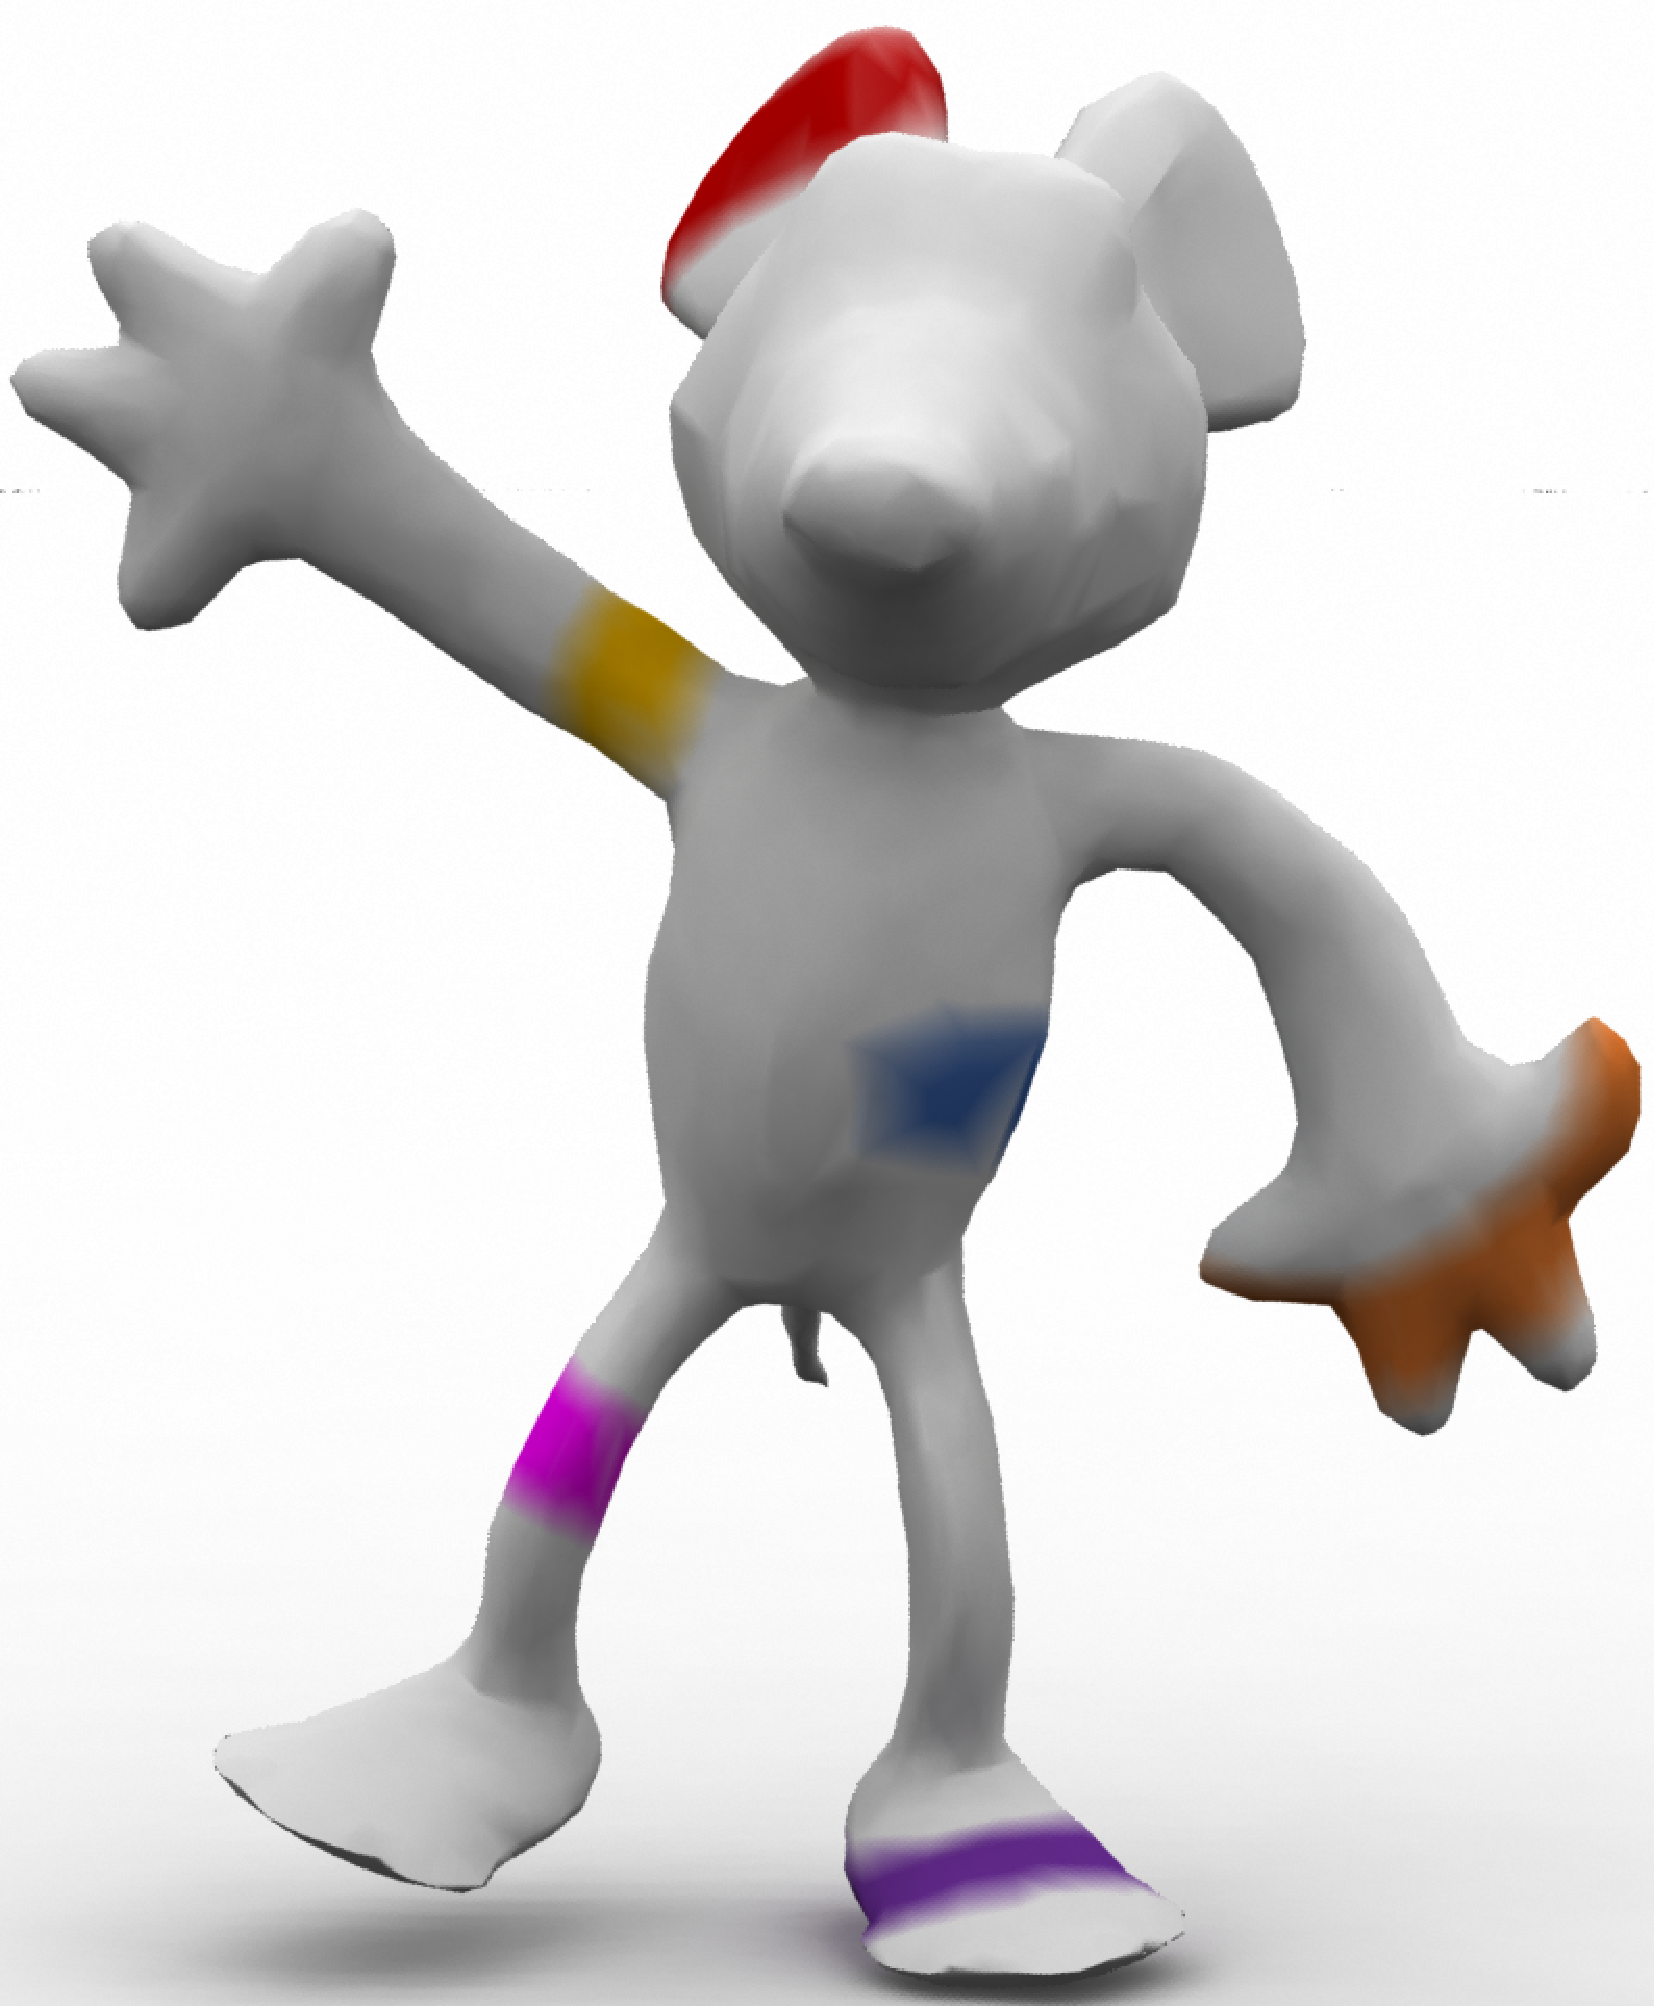
\includegraphics[height=.6\linewidth]{figures/symmetry/target_symmetric_mouse_cropped.pdf}\\
$\source$ & $\G'$
\end{tabular}
\vspace{-.17in}
\caption{Self symmetry.}\label{fig:self-symmetry}
\end{wrapfigure}
Figure~\ref{fig:self-symmetry} shows the more conventional case of intrinsic ``self''-symmetry detection.  In this case, we seek maps from the mouse model onto itself that preserve distance structure ($\alpha\!=\!10^{-3},\varepsilon\!=\!10^{-3}$).  To avoid the obvious identity map, we optimize for $\G'$ after taking $\G$ to be the identity matrix.  This yields the left-right symmetric map of the model.

Notice the construction of this technique relies upon the non-convexity of the \GWa objective.  In particular, averaging the orientation-preserving and orientation-reversing maps \emph{increases} the \GWa objective, a property that cannot hold for convex functions.

\subsection{Joint Domain Analysis}\label{sec:consistency}

%While the simplicity of Algorithm~\ref{alg:gw} is attractive, it does not enforce consistency.
A valuable property of mapping within a collection is \emph{consistency.} If we map $\mathcal A$ to $\mathcal B$, $\mathcal B$ to  $\mathcal C$, and  $\mathcal C$ back to  $\mathcal A$, we may wish to constrain the composition to approximate the identity.  Consistency can help improve a collection of maps by reinforcing correct matches.% and helping detect poor maps.

%\begin{figure}[t]
%\centering
%\graphicspath{ {figures/consistency_line_drawing/} }
%\begin{tabular}{cc}
%\def\svgwidth{.2\textwidth}\input{figures/consistency_line_drawing/pairwise_maps.pdf_tex}&
%\def\svgwidth{.18\textwidth}\input{figures/consistency_line_drawing/urshape.pdf_tex}\\
%Pairwise maps & Factoring through urshape
%\end{tabular}
%\caption{If a set of pairwise maps (left) is \emph{consistent}, they all can be factored through a single ``urshape.''  Pairwise maps are recovered by mapping from the source to the urshape and then from the urshape to the target.}\label{fig:urshape}
%\end{figure}

Suppose we are given domains $\{\mathcal D_1,\ldots,\mathcal D_p\}$ with pairwise couplings $\G\!_{ij}\in\bM(\bmu_i,\bmu_j);$ % that is, $\G\!_{ij}$ satisfies $\G\!_{ij}^\top\bmu_i=\1$ and $\G\!_{ij}\bmu_j=\1.$  
$\G\!_{ij}$ and $\G\!_{jk}$ can be composed as $\G\!_{ij}\diag{\bmu_{j}}\G\!_{jk}$ (see appendix).
Following~\cite{huang-2013}, % and in Figure~\ref{fig:urshape}, 
if the $\G\!_{ij}$'s are consistent, they factor through an ``urshape,'' that is, we could map every $\mathcal D_i$ to a single target and back out. If the urshape approximately consists of $m$ uniformly-sampled points, we can write $\G\!_1,\ldots,\G\!_p\in\bM(\bmu_i,\nicefrac{\1}{m})$ such that $\G\!_{ij}=\nicefrac{\G\!_i\G\!_j^\top}{m}:$ 
%Organizing the maps into a block matrix shows
\begin{equation}\label{eq:factor}
\underbrace{
\left(
\begin{array}{c@{\,}c@{\,}c}
\G\!_{11} & \cdots & \G\!_{1p}\\
\vdots & \ddots & \vdots\\
\G\!_{p1} & \cdots & \G\!_{pp}
\end{array}
\right)}_{\bG}
=\frac{1}{m}
\underbrace{\left(\begin{array}{c} \G\!_1 \\ \G\!_2 \\ \vdots \\ \G\!_p \end{array}\right)}_{\bA}
\underbrace{\left(\begin{array}{c} \G\!_1 \\ \G\!_2 \\ \vdots \\ \G\!_p \end{array}\right)^\top}_{\bA^\top}.
\end{equation}
%That is, if $\bG\in\R_+^{N\times N}$ is the matrix of pairwise couplings, then $\bG=\nicefrac{\bA\bA^\top}{m}$ for a matrix $\bA\in\R_+^{N\times m}$ of maps into the urshape.  
This shows that $\bG$ admits a \emph{low-rank, symmetric nonnegative factorization} proportional to $\bA\bA^\top$.  %In particular, $\bG$ can have rank at most $m$, with $m\ll N$ as the number of shapes grows; the factors are nonnegative measure couplings.  
%Note that while consistent mapping methods like~\cite{huang-2013,pachauri-2013,chen-2014} also include this low-rank assumption, the nonnegativity of $\bA$ further reduces our search space.

Suppose we are given metric matrices $\D_1,\ldots,\D_p$.  For simplicity, we assume $\D_i\in\R_+^{m\times m}\,\forall i$ with constant area weights.  From~\eqref{eq:factor}, we optimize for a set of nearly-consistent maps $\G\!_{ij}$ as follows:
\begin{equation}\label{eq:consistent_gw}
\begin{array}{r@{\ }l}
\min_{\bG,\bA} & \beta\KL(\bG|\bA\bA^\top)\!+\!\sum_{ij} \KL(\G\!_{ij}|\f_\alpha(\G\!_{ij};\D_i,\D_j))\\
\textrm{s.t.} & \bG\textrm{ has blocks }\G\!_{ij}\textrm{ and }\bA\textrm{ has blocks }\G\!_i\\
& \G\!_{ij},\G\!_i\in\bM(\nicefrac{\1}{m},\nicefrac{\1}{m})\ \forall i,j
\end{array}
\end{equation}
The second term is the \GWa objective~\eqref{eq:reg_gw}, and the first approximates $\bG$ as $\bA\bA^\top$.  This resembles factorizations in probabilistic latent semantic analysis (pLSA)~\cite{hofmann-1999}, which approximate $\bB\approx\bW\bH$ %for low-rank and nonnegative $\bW,\bH$ 
by minimizing $\KL(\bB|\bW\bH)$~\cite{gaussier-2005}.   % $\bW,\bH$ appear on the right-hand side of KL divergence, while Algorithm~\ref{alg:gw}  deals with the left-hand side of KL divergence, motivating the construction in~\eqref{eq:consistent_gw}.

%\subsubsection{Optimization}

We minimize~\eqref{eq:consistent_gw} by alternating between $\bG$ and $\bA$.  Each alternation has a straightforward algorithm detailed below and in Algorithm~\ref{alg:consistent_gw}.  Our method ensures that the objective of~\eqref{eq:consistent_gw} decreases in each step, but we leave to future work a result like Proposition~\ref{prop:gw_convergence}.%; the method is detailed in Algorithm~\ref{alg:consistent_gw}.

%\paragraph{Map computation.}

First, suppose $\bA$ is fixed and that we optimize for $\bG$.  %This problem deals with the \emph{left} side of KL divergence.
Denote by $\F_\alpha(\bG)$ the matrix with blocks $\f_\alpha(\G\!_{ij};\D_i,\D_j)$.  Algebraic manipulation of~\eqref{eq:consistent_gw} with $\bA$ fixed yields an equivalent problem
\begin{equation}\label{eq:consistent_gw_merged}
\begin{array}{r@{\ }l}
\min_{\bG} & \KL\left(\bG\left|\F_\alpha(\bG)^{\wedge(1-\delta)}\otimes(\bA\bA^\top)^{\wedge\delta}\right.\right)\\
\textrm{s.t.} & \bG\textrm{ has blocks }\G\!_{ij}\textrm{ and }\bA\textrm{ has blocks }\G\!_i\\
& \G\!_{ij},\G\!_i\in\bM(\nicefrac{\1}{m},\nicefrac{\1}{m})\ \forall i,j,
\end{array}
\end{equation}
where $\delta\eqdef\nicefrac{1}{1+\beta}.$  Problem~\eqref{eq:consistent_gw_merged} decouples over the $m\!\times\!m$ blocks of $\bG$, and each individual problem is an instance of the \GWa objective with elementwise scaling from $\bA\bA^\top$.

%\paragraph{Low-rank factorization.} 

\begin{algorithm}[t]
\fbox{\hspace{-.1in}\parbox{\columnwidth}{%
\begin{algorithmic}
\Function{Symmetric-NNMF}{$\bB$}
%	\LineComment{Nonnegative matrix factorization $\bB\approx\bA\bA^\top$}
%	\algspace
	\Let{$\bA$}{\Call{Random}{$pm\times m$}}\Comment{Initialize with nontrivial $\bA$}
	\For{$\ell=1,2,3,\ldots$}
		\Let{$\bU$}{$\bA\otimes[(\bB\oslash \bA\bA^\top)\bA]$}
		\Let{$\bA$}{$\bU\diag{\1\oslash\sqrt{\bU^\top\1}}$}
	\EndFor
	\State\Return{$\bA$}\Comment{$\bB\approx\bA\bA^\top$}
\EndFunction
  \end{algorithmic}
}}
\vspace{-3mm}
\caption{Nonnegative matrix factorization minimizing $\KL(\bB|\bA\bA^\top)$ with respect to $\bA$.\vspace{-.15in}}\label{alg:nnmf}
\end{algorithm}

Now, suppose $\bG$ is fixed, leaving minimization of $\KL(\bG|\bA\bA^\top)$ with respect to $\bA$.  Unlike pLSA, we factor $\bG\approx \bA\bA^\top$ rather than $\bA\approx\bW\bH$.  We minimize with respect to a \emph{single} $\bA$ rather than minimizing $\KL(\bG|\bW\bH)$ over $\bW$ and $\bH$ independently.  Algorithm~\ref{alg:nnmf} provides a simple iteration for this factorization, using majorization-minimization~\cite{hunter-2000}.  We prove the following monotonicity property in the appendix:

\begin{proposition}\label{prop:nnmf_monotonicity}
Denote the iterates of Algorithm~\ref{alg:nnmf} as $\bA\!^{(\ell)}.$  Then, $\KL(\bG|\bA\!^{(\ell)}\bA\!^{(\ell)\top})$ decreases as a function of $\ell$, with monotonicity unless $\bA\!^{(\ell)}$ is a critical point of $\KL(\bG|\bA\bA^\top)$.
\end{proposition}
%It is weaker than Proposition~\ref{prop:gw_convergence} in that we show convergence of the objective rather than the iterates.  
The work of~\cite{lanckriet-2009} might be used to obtain more refined convergence results.% results; we leave this analysis to future work.

%\paragraph*{Outer loop.}

\begin{algorithm}[t]
\fbox{\hspace{-.1in}\parbox{\columnwidth}{%
\begin{algorithmic}
\Function{Joint-$\GWa$}{$\D_1,\ldots,\D_p;\delta,\eta$}
	\LineComment{Computes consistent maps via~\eqref{eq:consistent_gw_merged}.}
	\algspace
	\Let{$\bA$}{\Call{Ones}{$pm\times m$}}
	\Let{$\bG$}{\Call{Ones}{$pm\times pm$}}
	\For{$k=1,2,3,\ldots$}
		\Let{$\bG_0$}{$\frac{1}{m}\bA\bA^\top$}\Comment{Consistent pairwise maps}
		\For{$i,j=1,2,\ldots,p$}\Comment{Fix $\bA$ and optimize $\bG$}
			\Let{$\G\!_{ij}$}{\Call{Block-Projection}{$\D_i,\D_j,(\bG_0)_{ij};\delta,\eta$}}
			\Let{\Call{Block}{$\bG,i,j$}}{$\G\!_{ij}$}\Comment{Replace block of $\bG$}
		\EndFor
		\Let{$\bA$}{\Call{Symmetric-NNMF}{$\bG^{\wedge(1/\delta)}\otimes \F_\alpha(\bG)^{\wedge(1-1/\delta)}$}}
	\EndFor
	\algspace
	\State\Return{$(\bA,\bG)$}
\EndFunction
  \end{algorithmic}
}}
\algspace\\
\fbox{\hspace{-.1in}\parbox{\columnwidth}{%
\begin{algorithmic}
\Function{Block-Projection}{$\D_i,\D_j,\bV;\delta,\eta$}
	\LineComment{Blockwise projection for consistent GW}
	\algspace
	\Let{$\G$}{\Call{Ones}{$m\times m$}}
	\For{$\ell=1,2,3,\ldots$}
		\Let{$\K$}{$\f_\alpha(\G)^{\wedge(1-\delta)}\otimes\bV^{\wedge \delta}$}	
		\Let{$\G$}{\Call{Sinkhorn-Projection}{$\K^{\wedge\!\eta}\otimes\G^{\wedge\!(1\!-\!\eta)}\!;\frac{\1}{m},\frac{\1}{m}$}}
	\EndFor
	\State\Return{$\G$}
\EndFunction
  \end{algorithmic}
}}
\vspace{-3mm}
\caption{Algorithm for joint GW matching.}\label{alg:consistent_gw}
\end{algorithm}

% summarizes our consistent matching algorithm, which alternates between the two steps above.  In practice, reusing $\bA,\bG$ from previous iterations to future iterations can speed convergence of the inner nonnegative matrix factorization and Gromov-Wasserstein loops.  This alternation is guaranteed to decrease the objective~\eqref{eq:consistent_gw} in each step.

%\subsubsection{Examples}

%\justin{Examples of consistent maps.}

%\justin{Note that the factorization algorithm is new, maybe compare with Peter's SDP.}

%\justin{TODO:  Rewrite with lower rank.}

\begin{figure}[t]\centering
$\begin{array}{l}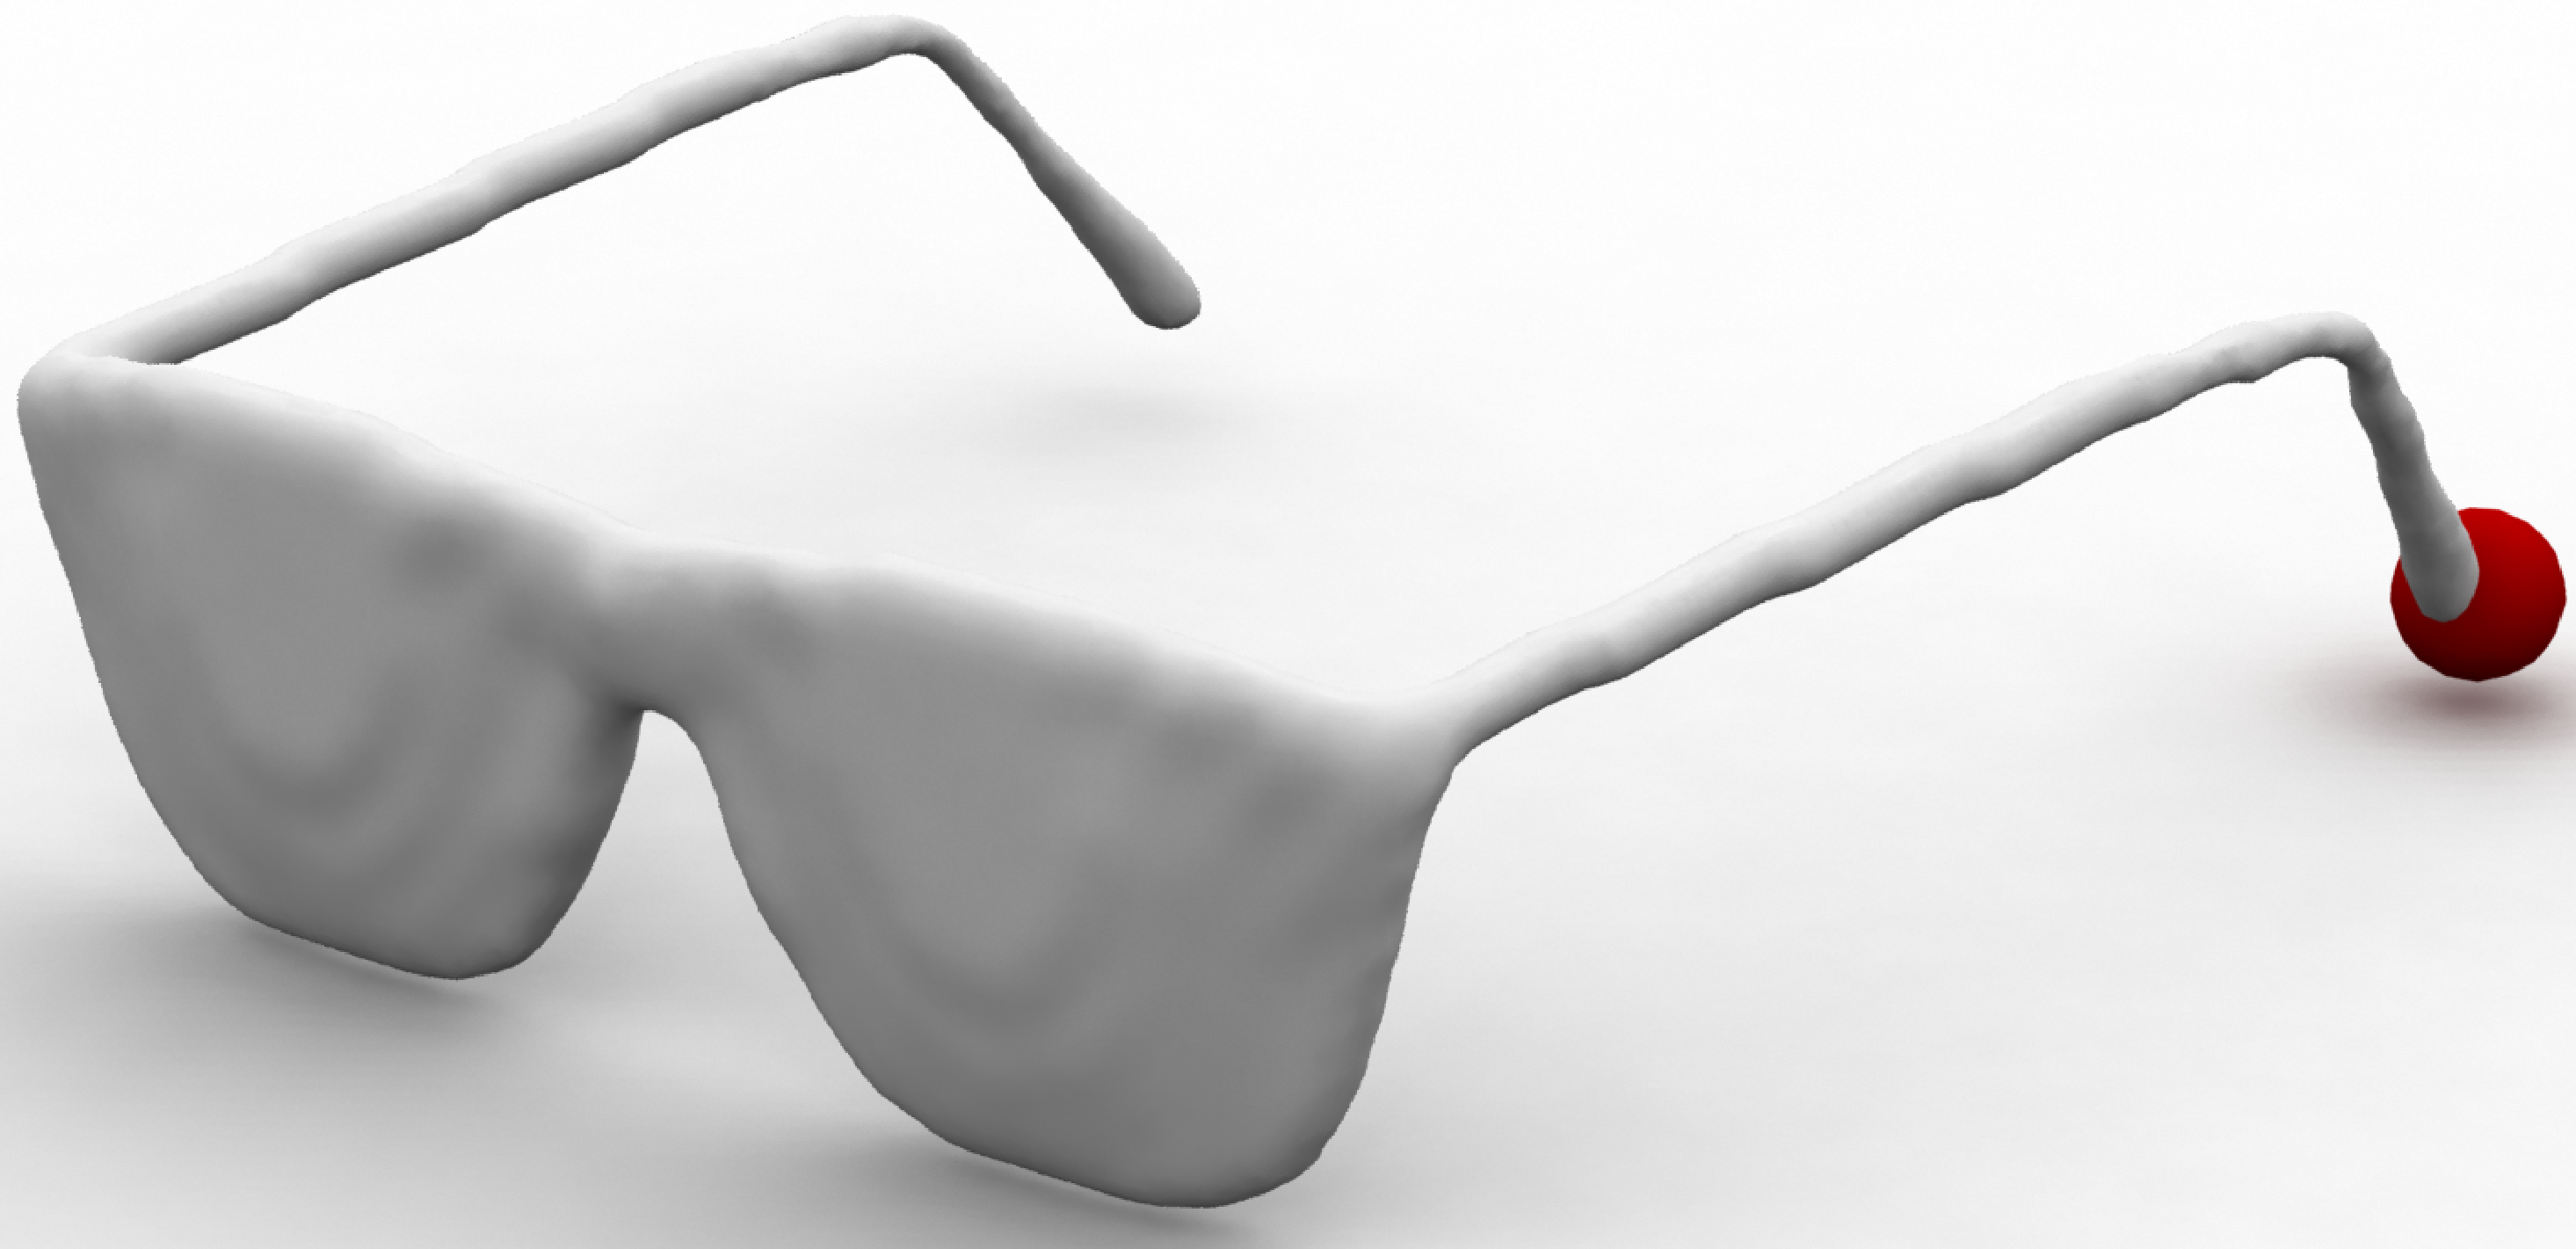
\includegraphics[width=.2\linewidth]{figures/consistent_maps/source_point.pdf}\end{array}$ \textrm{\small Source point} \\
\begin{tabular}{@{}c@{}c@{}}
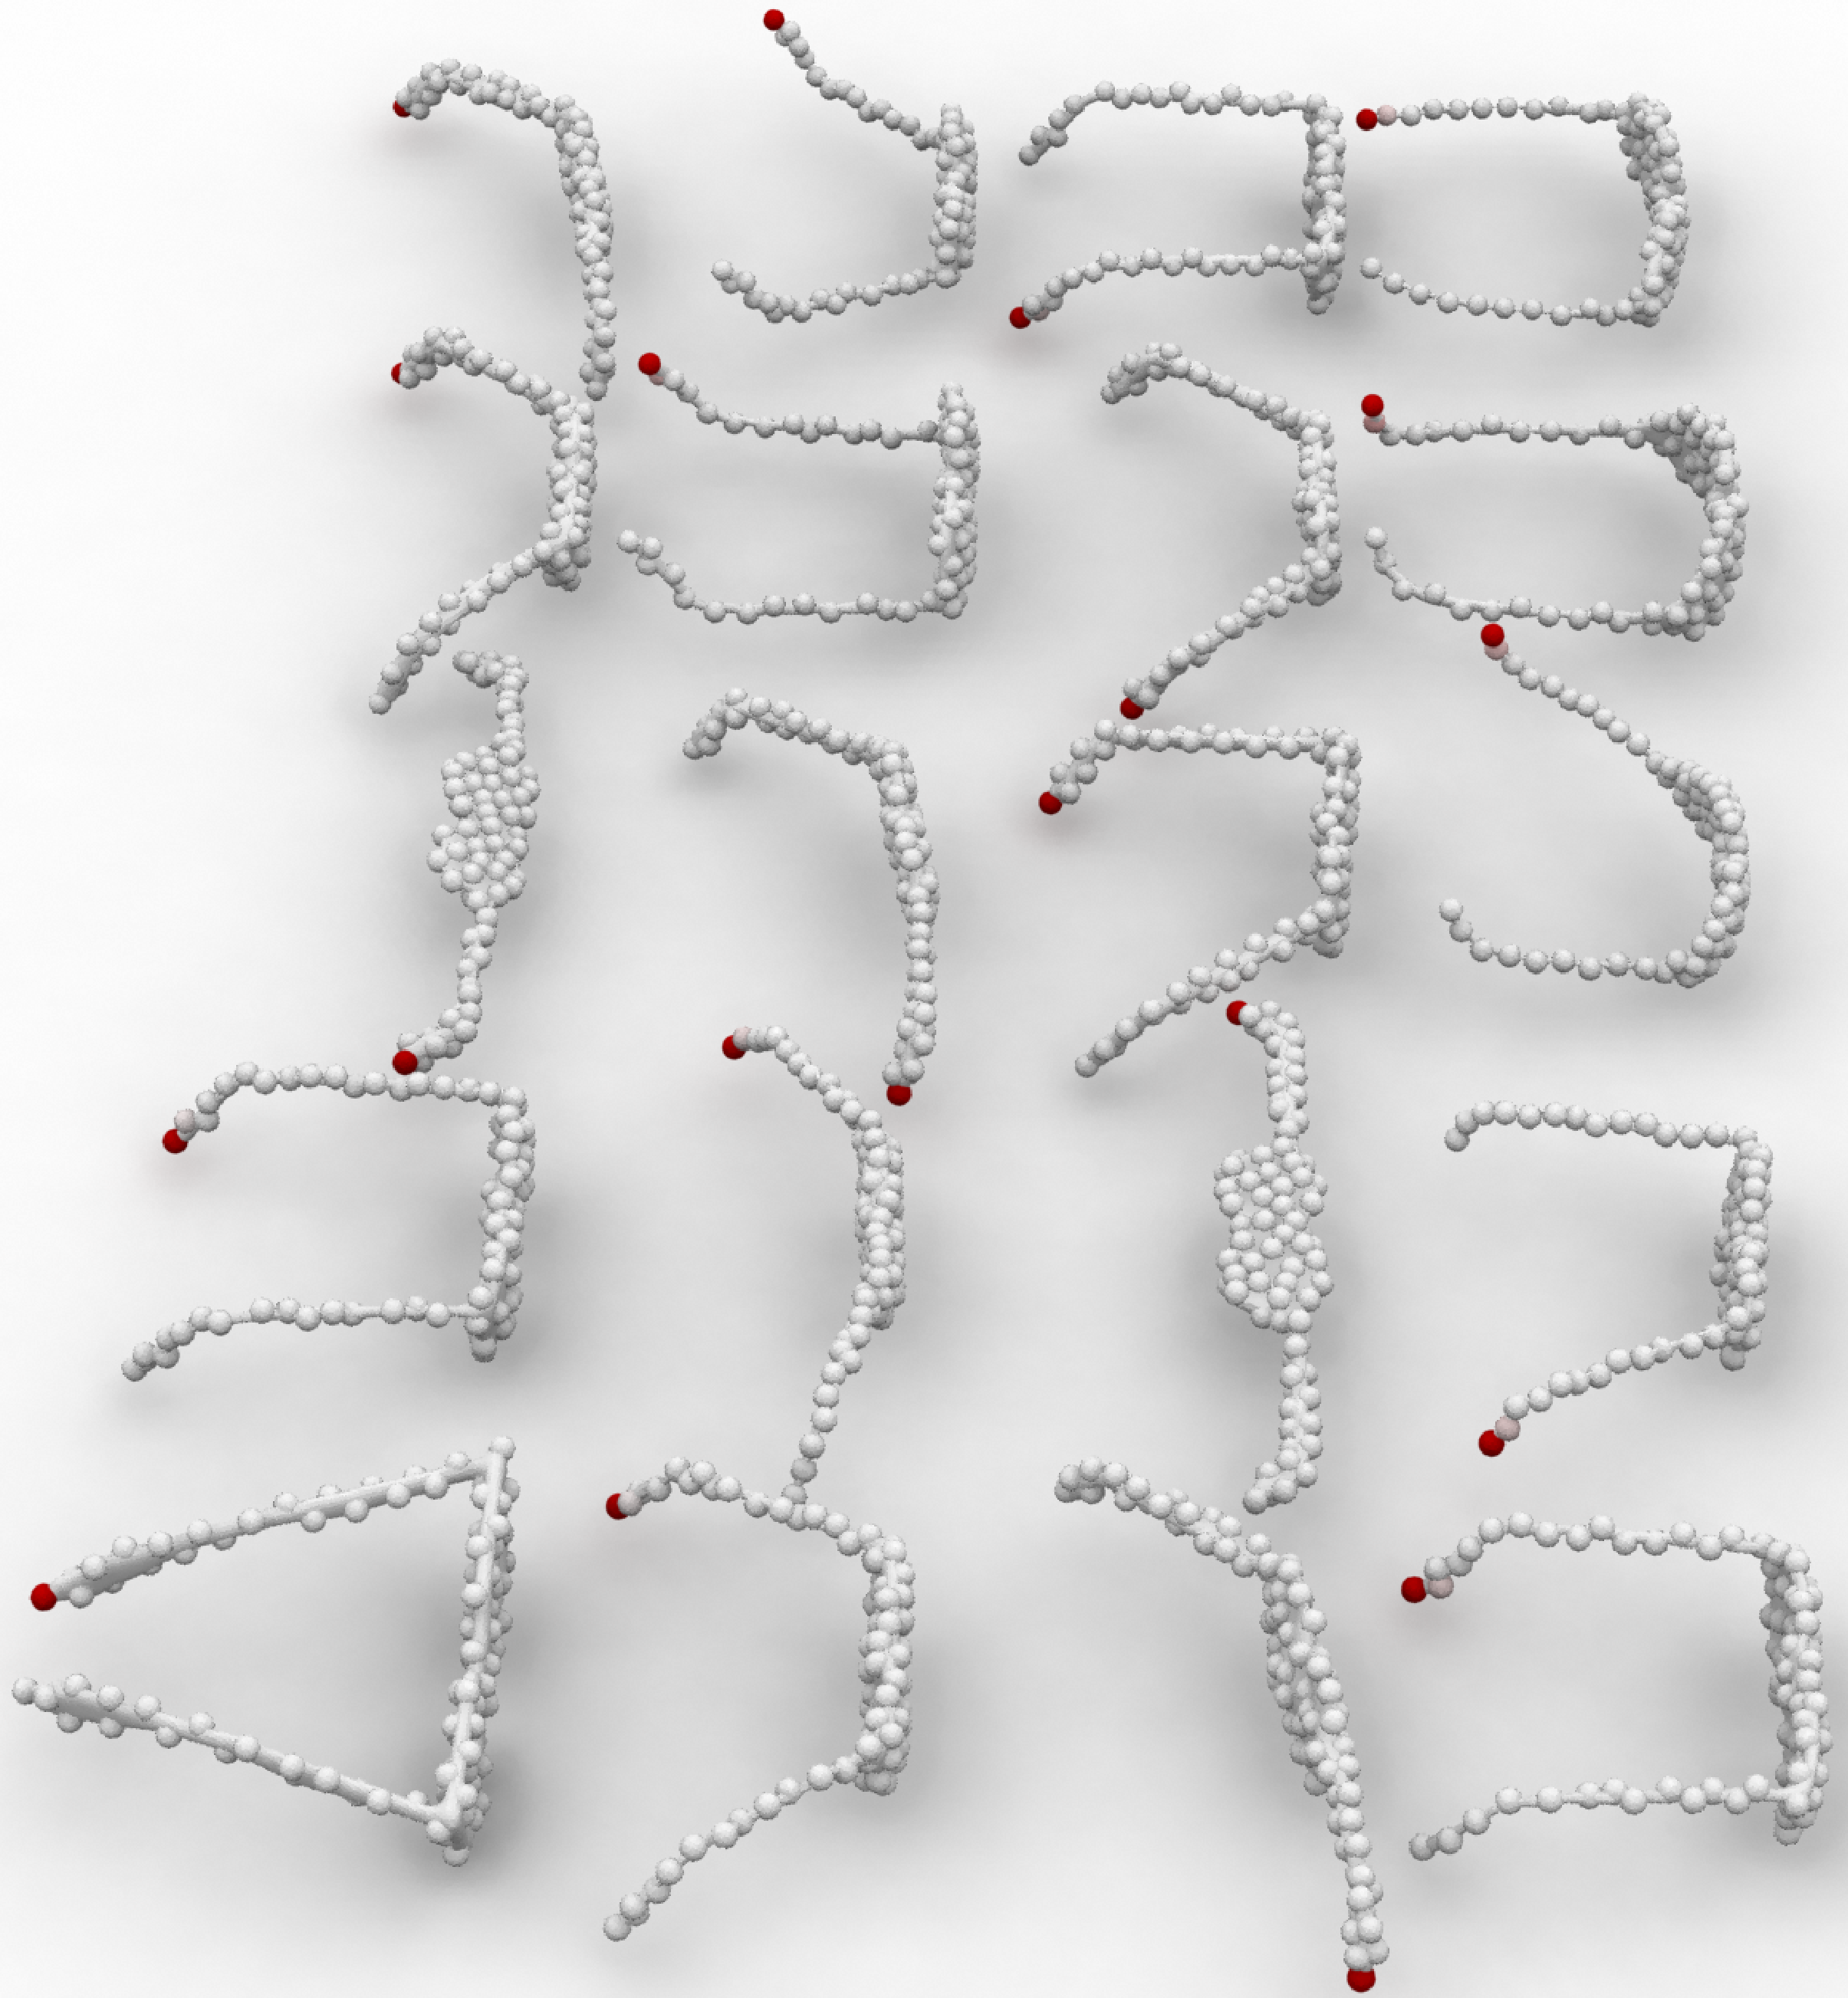
\includegraphics[width=.5\linewidth]{figures/consistent_maps/target_inconsistent_cropped.pdf}&
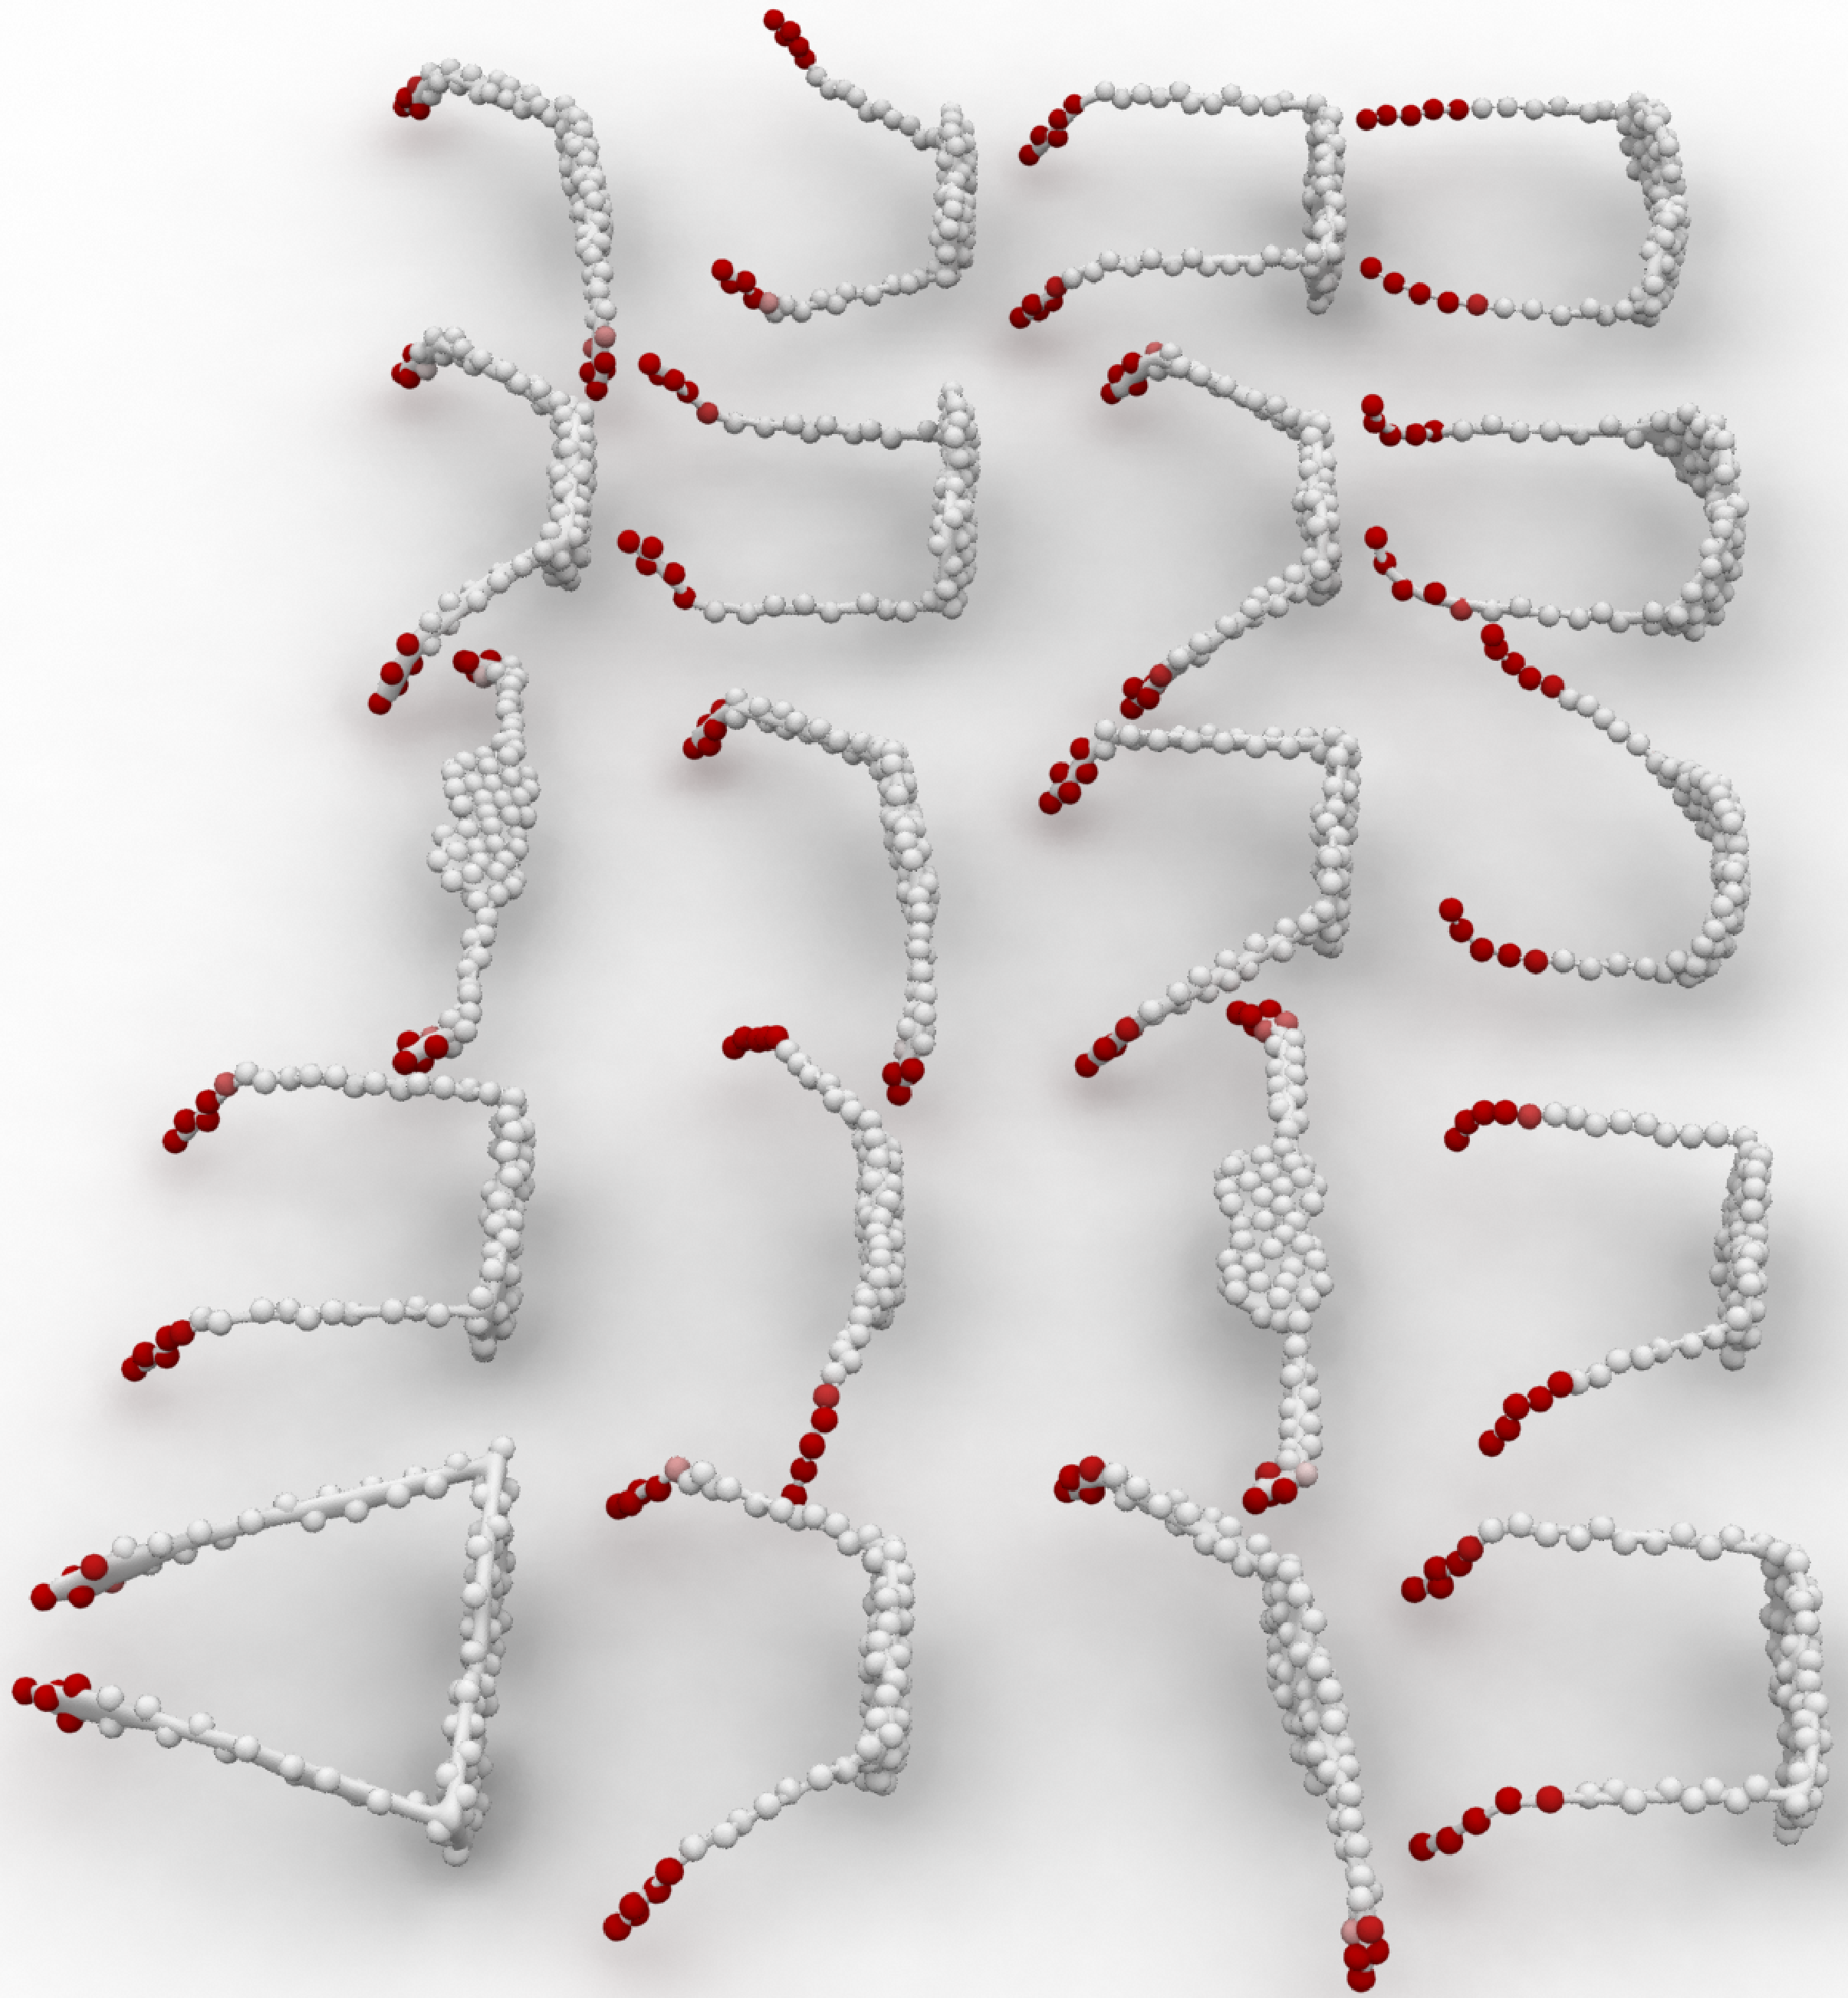
\includegraphics[width=.5\linewidth]{figures/consistent_maps/target_consistent_cropped.pdf}\\
Inconsistent & Consistent
\end{tabular}
\caption{Consistent mapping via low-rank factorization reveals the left-right symmetric ambiguity of mapping between twenty models of eyeglasses ($\alpha=10^{-3},\beta=1$, $n=100$, rank 15).\vspace{-.15in}}\label{fig:consistent_gw}
\end{figure}
Figure~\ref{fig:consistent_gw} illustrates an example of consistent mapping using the technique outlined above.  In this case, we compute consistent maps between 20 models of eyeglasses, each sampled with 100 points.  Pairwise mapping using the \GWa objective yields maps with arbitrary, inconsistent left-right flips.  Adding the low-rank term~\eqref{eq:consistent_gw} produces maps that superpose the ambiguous symmetry.  For this experiment, we take $A$ to be rank 15; this choice of dimensionality accelerates convergence of the alternating algorithm and is reasonable given the symmetry we expect in the final maps.


%%% Local Variables:
%%% mode: latex
%%% TeX-master: "../gw"
%%% End:
